% Options for packages loaded elsewhere
\PassOptionsToPackage{unicode}{hyperref}
\PassOptionsToPackage{hyphens}{url}
%
\documentclass[
]{article}
\usepackage{amsmath,amssymb}
\usepackage{lmodern}
\usepackage{ifxetex,ifluatex}
\ifnum 0\ifxetex 1\fi\ifluatex 1\fi=0 % if pdftex
  \usepackage[T1]{fontenc}
  \usepackage[utf8]{inputenc}
  \usepackage{textcomp} % provide euro and other symbols
\else % if luatex or xetex
  \usepackage{unicode-math}
  \defaultfontfeatures{Scale=MatchLowercase}
  \defaultfontfeatures[\rmfamily]{Ligatures=TeX,Scale=1}
\fi
% Use upquote if available, for straight quotes in verbatim environments
\IfFileExists{upquote.sty}{\usepackage{upquote}}{}
\IfFileExists{microtype.sty}{% use microtype if available
  \usepackage[]{microtype}
  \UseMicrotypeSet[protrusion]{basicmath} % disable protrusion for tt fonts
}{}
\makeatletter
\@ifundefined{KOMAClassName}{% if non-KOMA class
  \IfFileExists{parskip.sty}{%
    \usepackage{parskip}
  }{% else
    \setlength{\parindent}{0pt}
    \setlength{\parskip}{6pt plus 2pt minus 1pt}}
}{% if KOMA class
  \KOMAoptions{parskip=half}}
\makeatother
\usepackage{xcolor}
\IfFileExists{xurl.sty}{\usepackage{xurl}}{} % add URL line breaks if available
\IfFileExists{bookmark.sty}{\usepackage{bookmark}}{\usepackage{hyperref}}
\hypersetup{
  pdftitle={8\_Vis\_IS\_results},
  pdfauthor={Kurt Ingeman},
  hidelinks,
  pdfcreator={LaTeX via pandoc}}
\urlstyle{same} % disable monospaced font for URLs
\usepackage[margin=1in]{geometry}
\usepackage{color}
\usepackage{fancyvrb}
\newcommand{\VerbBar}{|}
\newcommand{\VERB}{\Verb[commandchars=\\\{\}]}
\DefineVerbatimEnvironment{Highlighting}{Verbatim}{commandchars=\\\{\}}
% Add ',fontsize=\small' for more characters per line
\usepackage{framed}
\definecolor{shadecolor}{RGB}{248,248,248}
\newenvironment{Shaded}{\begin{snugshade}}{\end{snugshade}}
\newcommand{\AlertTok}[1]{\textcolor[rgb]{0.94,0.16,0.16}{#1}}
\newcommand{\AnnotationTok}[1]{\textcolor[rgb]{0.56,0.35,0.01}{\textbf{\textit{#1}}}}
\newcommand{\AttributeTok}[1]{\textcolor[rgb]{0.77,0.63,0.00}{#1}}
\newcommand{\BaseNTok}[1]{\textcolor[rgb]{0.00,0.00,0.81}{#1}}
\newcommand{\BuiltInTok}[1]{#1}
\newcommand{\CharTok}[1]{\textcolor[rgb]{0.31,0.60,0.02}{#1}}
\newcommand{\CommentTok}[1]{\textcolor[rgb]{0.56,0.35,0.01}{\textit{#1}}}
\newcommand{\CommentVarTok}[1]{\textcolor[rgb]{0.56,0.35,0.01}{\textbf{\textit{#1}}}}
\newcommand{\ConstantTok}[1]{\textcolor[rgb]{0.00,0.00,0.00}{#1}}
\newcommand{\ControlFlowTok}[1]{\textcolor[rgb]{0.13,0.29,0.53}{\textbf{#1}}}
\newcommand{\DataTypeTok}[1]{\textcolor[rgb]{0.13,0.29,0.53}{#1}}
\newcommand{\DecValTok}[1]{\textcolor[rgb]{0.00,0.00,0.81}{#1}}
\newcommand{\DocumentationTok}[1]{\textcolor[rgb]{0.56,0.35,0.01}{\textbf{\textit{#1}}}}
\newcommand{\ErrorTok}[1]{\textcolor[rgb]{0.64,0.00,0.00}{\textbf{#1}}}
\newcommand{\ExtensionTok}[1]{#1}
\newcommand{\FloatTok}[1]{\textcolor[rgb]{0.00,0.00,0.81}{#1}}
\newcommand{\FunctionTok}[1]{\textcolor[rgb]{0.00,0.00,0.00}{#1}}
\newcommand{\ImportTok}[1]{#1}
\newcommand{\InformationTok}[1]{\textcolor[rgb]{0.56,0.35,0.01}{\textbf{\textit{#1}}}}
\newcommand{\KeywordTok}[1]{\textcolor[rgb]{0.13,0.29,0.53}{\textbf{#1}}}
\newcommand{\NormalTok}[1]{#1}
\newcommand{\OperatorTok}[1]{\textcolor[rgb]{0.81,0.36,0.00}{\textbf{#1}}}
\newcommand{\OtherTok}[1]{\textcolor[rgb]{0.56,0.35,0.01}{#1}}
\newcommand{\PreprocessorTok}[1]{\textcolor[rgb]{0.56,0.35,0.01}{\textit{#1}}}
\newcommand{\RegionMarkerTok}[1]{#1}
\newcommand{\SpecialCharTok}[1]{\textcolor[rgb]{0.00,0.00,0.00}{#1}}
\newcommand{\SpecialStringTok}[1]{\textcolor[rgb]{0.31,0.60,0.02}{#1}}
\newcommand{\StringTok}[1]{\textcolor[rgb]{0.31,0.60,0.02}{#1}}
\newcommand{\VariableTok}[1]{\textcolor[rgb]{0.00,0.00,0.00}{#1}}
\newcommand{\VerbatimStringTok}[1]{\textcolor[rgb]{0.31,0.60,0.02}{#1}}
\newcommand{\WarningTok}[1]{\textcolor[rgb]{0.56,0.35,0.01}{\textbf{\textit{#1}}}}
\usepackage{graphicx}
\makeatletter
\def\maxwidth{\ifdim\Gin@nat@width>\linewidth\linewidth\else\Gin@nat@width\fi}
\def\maxheight{\ifdim\Gin@nat@height>\textheight\textheight\else\Gin@nat@height\fi}
\makeatother
% Scale images if necessary, so that they will not overflow the page
% margins by default, and it is still possible to overwrite the defaults
% using explicit options in \includegraphics[width, height, ...]{}
\setkeys{Gin}{width=\maxwidth,height=\maxheight,keepaspectratio}
% Set default figure placement to htbp
\makeatletter
\def\fps@figure{htbp}
\makeatother
\setlength{\emergencystretch}{3em} % prevent overfull lines
\providecommand{\tightlist}{%
  \setlength{\itemsep}{0pt}\setlength{\parskip}{0pt}}
\setcounter{secnumdepth}{-\maxdimen} % remove section numbering
\ifluatex
  \usepackage{selnolig}  % disable illegal ligatures
\fi

\title{8\_Vis\_IS\_results}
\author{Kurt Ingeman}
\date{6/27/2021}

\begin{document}
\maketitle

\begin{Shaded}
\begin{Highlighting}[]
\FunctionTok{rm}\NormalTok{(}\AttributeTok{list =} \FunctionTok{ls}\NormalTok{())}

\FunctionTok{library}\NormalTok{(here)}
\end{Highlighting}
\end{Shaded}

\begin{verbatim}
## here() starts at /Users/kurtingeman/github/CORE
\end{verbatim}

\begin{Shaded}
\begin{Highlighting}[]
\FunctionTok{library}\NormalTok{(tidyr)}
\FunctionTok{library}\NormalTok{(dplyr)}
\end{Highlighting}
\end{Shaded}

\begin{verbatim}
## 
## Attaching package: 'dplyr'
\end{verbatim}

\begin{verbatim}
## The following objects are masked from 'package:stats':
## 
##     filter, lag
\end{verbatim}

\begin{verbatim}
## The following objects are masked from 'package:base':
## 
##     intersect, setdiff, setequal, union
\end{verbatim}

\begin{Shaded}
\begin{Highlighting}[]
\FunctionTok{library}\NormalTok{(ggplot2)}
\FunctionTok{library}\NormalTok{(fmsb)}
\FunctionTok{library}\NormalTok{(forcats)}
\FunctionTok{library}\NormalTok{(RColorBrewer)}
\end{Highlighting}
\end{Shaded}

\begin{Shaded}
\begin{Highlighting}[]
\FunctionTok{load}\NormalTok{(}\FunctionTok{here}\NormalTok{(}\StringTok{"CORE EDM analysis"}\NormalTok{, }\StringTok{"Output"}\NormalTok{, }\StringTok{"Rdata"}\NormalTok{, }\StringTok{"4\_IS"}\NormalTok{, }\StringTok{"SMAP\_best\_embeddings\_ESU\_rec4n.RData"}\NormalTok{)) }
\NormalTok{rec4\_ESU }\OtherTok{\textless{}{-}}\NormalTok{ out\_results}
\FunctionTok{rm}\NormalTok{(out\_results)}

\FunctionTok{load}\NormalTok{(}\FunctionTok{here}\NormalTok{(}\StringTok{"CORE EDM analysis"}\NormalTok{, }\StringTok{"Output"}\NormalTok{, }\StringTok{"Rdata"}\NormalTok{, }\StringTok{"4\_IS"}\NormalTok{, }\StringTok{"SMAP\_best\_embeddings\_Imnaha\_rec4n.RData"}\NormalTok{)) }
\NormalTok{rec4\_IMN }\OtherTok{\textless{}{-}}\NormalTok{ out\_results}
\FunctionTok{rm}\NormalTok{(out\_results)}

\FunctionTok{load}\NormalTok{(}\FunctionTok{here}\NormalTok{(}\StringTok{"CORE EDM analysis"}\NormalTok{, }\StringTok{"Output"}\NormalTok{, }\StringTok{"Rdata"}\NormalTok{, }\StringTok{"4\_IS"}\NormalTok{, }\StringTok{"SMAP\_best\_embeddings\_Middle Fork Salmon\_rec4n.RData"}\NormalTok{)) }
\NormalTok{rec4\_MFS }\OtherTok{\textless{}{-}}\NormalTok{ out\_results}
\FunctionTok{rm}\NormalTok{(out\_results)}

\FunctionTok{load}\NormalTok{(}\FunctionTok{here}\NormalTok{(}\StringTok{"CORE EDM analysis"}\NormalTok{, }\StringTok{"Output"}\NormalTok{, }\StringTok{"Rdata"}\NormalTok{, }\StringTok{"4\_IS"}\NormalTok{, }\StringTok{"SMAP\_best\_embeddings\_Upper Salmon\_rec4n.RData"}\NormalTok{)) }
\NormalTok{rec4\_UPS }\OtherTok{\textless{}{-}}\NormalTok{ out\_results}
\FunctionTok{rm}\NormalTok{(out\_results)}
\end{Highlighting}
\end{Shaded}

\hypertarget{create-domains-ocean-human-predator}{%
\subsection{create domains (Ocean, Human,
Predator)}\label{create-domains-ocean-human-predator}}

\begin{Shaded}
\begin{Highlighting}[]
\NormalTok{rec4\_ESU}\OtherTok{\textless{}{-}}\NormalTok{  rec4\_ESU }\SpecialCharTok{\%\textgreater{}\%} 
  \FunctionTok{mutate}\NormalTok{(}\AttributeTok{domain =} \FunctionTok{case\_when}\NormalTok{(}
    \FunctionTok{grepl}\NormalTok{(}\StringTok{"npgo"}\NormalTok{, FP) }\SpecialCharTok{\textasciitilde{}} \StringTok{"ocean"}\NormalTok{,}
    \FunctionTok{grepl}\NormalTok{(}\StringTok{"pdo"}\NormalTok{, FP) }\SpecialCharTok{\textasciitilde{}} \StringTok{"ocean"}\NormalTok{,}
    \FunctionTok{grepl}\NormalTok{(}\StringTok{"arc"}\NormalTok{, FP) }\SpecialCharTok{\textasciitilde{}} \StringTok{"ocean"}\NormalTok{,}
    \FunctionTok{grepl}\NormalTok{(}\StringTok{"upw"}\NormalTok{, FP) }\SpecialCharTok{\textasciitilde{}} \StringTok{"ocean"}\NormalTok{, }
    \FunctionTok{grepl}\NormalTok{(}\StringTok{"hatch"}\NormalTok{, FP) }\SpecialCharTok{\textasciitilde{}} \StringTok{"human"}\NormalTok{,}
    \FunctionTok{grepl}\NormalTok{(}\StringTok{"harv"}\NormalTok{, FP) }\SpecialCharTok{\textasciitilde{}} \StringTok{"human"}\NormalTok{,}
    \FunctionTok{grepl}\NormalTok{(}\StringTok{"hseal"}\NormalTok{, FP) }\SpecialCharTok{\textasciitilde{}} \StringTok{"pred"}\NormalTok{,}
    \FunctionTok{grepl}\NormalTok{(}\StringTok{"orca"}\NormalTok{, FP) }\SpecialCharTok{\textasciitilde{}} \StringTok{"pred"}\NormalTok{,}
    \FunctionTok{grepl}\NormalTok{(}\StringTok{"csl"}\NormalTok{, FP) }\SpecialCharTok{\textasciitilde{}} \StringTok{"pred"}\NormalTok{, }
    \FunctionTok{grepl}\NormalTok{(}\StringTok{"ssl"}\NormalTok{, FP) }\SpecialCharTok{\textasciitilde{}} \StringTok{"pred"}\NormalTok{, }
    \ConstantTok{TRUE} \SpecialCharTok{\textasciitilde{}}\StringTok{"other"}\NormalTok{))}


\NormalTok{rec4\_IMN}\OtherTok{\textless{}{-}}\NormalTok{  rec4\_IMN }\SpecialCharTok{\%\textgreater{}\%} 
  \FunctionTok{mutate}\NormalTok{(}\AttributeTok{domain =} \FunctionTok{case\_when}\NormalTok{(}
    \FunctionTok{grepl}\NormalTok{(}\StringTok{"npgo"}\NormalTok{, FP) }\SpecialCharTok{\textasciitilde{}} \StringTok{"ocean"}\NormalTok{,}
    \FunctionTok{grepl}\NormalTok{(}\StringTok{"pdo"}\NormalTok{, FP) }\SpecialCharTok{\textasciitilde{}} \StringTok{"ocean"}\NormalTok{,}
    \FunctionTok{grepl}\NormalTok{(}\StringTok{"arc"}\NormalTok{, FP) }\SpecialCharTok{\textasciitilde{}} \StringTok{"ocean"}\NormalTok{,}
    \FunctionTok{grepl}\NormalTok{(}\StringTok{"upw"}\NormalTok{, FP) }\SpecialCharTok{\textasciitilde{}} \StringTok{"ocean"}\NormalTok{, }
    \FunctionTok{grepl}\NormalTok{(}\StringTok{"hatch"}\NormalTok{, FP) }\SpecialCharTok{\textasciitilde{}} \StringTok{"human"}\NormalTok{,}
    \FunctionTok{grepl}\NormalTok{(}\StringTok{"harv"}\NormalTok{, FP) }\SpecialCharTok{\textasciitilde{}} \StringTok{"human"}\NormalTok{,}
    \FunctionTok{grepl}\NormalTok{(}\StringTok{"hseal"}\NormalTok{, FP) }\SpecialCharTok{\textasciitilde{}} \StringTok{"pred"}\NormalTok{,}
    \FunctionTok{grepl}\NormalTok{(}\StringTok{"orca"}\NormalTok{, FP) }\SpecialCharTok{\textasciitilde{}} \StringTok{"pred"}\NormalTok{,}
    \FunctionTok{grepl}\NormalTok{(}\StringTok{"csl"}\NormalTok{, FP) }\SpecialCharTok{\textasciitilde{}} \StringTok{"pred"}\NormalTok{, }
    \FunctionTok{grepl}\NormalTok{(}\StringTok{"ssl"}\NormalTok{, FP) }\SpecialCharTok{\textasciitilde{}} \StringTok{"pred"}\NormalTok{, }
    \ConstantTok{TRUE} \SpecialCharTok{\textasciitilde{}}\StringTok{"other"}\NormalTok{))}

\NormalTok{rec4\_MFS }\OtherTok{\textless{}{-}}\NormalTok{  rec4\_MFS }\SpecialCharTok{\%\textgreater{}\%} 
  \FunctionTok{mutate}\NormalTok{(}\AttributeTok{domain =} \FunctionTok{case\_when}\NormalTok{(}
    \FunctionTok{grepl}\NormalTok{(}\StringTok{"npgo"}\NormalTok{, FP) }\SpecialCharTok{\textasciitilde{}} \StringTok{"ocean"}\NormalTok{,}
    \FunctionTok{grepl}\NormalTok{(}\StringTok{"pdo"}\NormalTok{, FP) }\SpecialCharTok{\textasciitilde{}} \StringTok{"ocean"}\NormalTok{,}
    \FunctionTok{grepl}\NormalTok{(}\StringTok{"arc"}\NormalTok{, FP) }\SpecialCharTok{\textasciitilde{}} \StringTok{"ocean"}\NormalTok{,}
    \FunctionTok{grepl}\NormalTok{(}\StringTok{"upw"}\NormalTok{, FP) }\SpecialCharTok{\textasciitilde{}} \StringTok{"ocean"}\NormalTok{, }
    \FunctionTok{grepl}\NormalTok{(}\StringTok{"hatch"}\NormalTok{, FP) }\SpecialCharTok{\textasciitilde{}} \StringTok{"human"}\NormalTok{,}
    \FunctionTok{grepl}\NormalTok{(}\StringTok{"harv"}\NormalTok{, FP) }\SpecialCharTok{\textasciitilde{}} \StringTok{"human"}\NormalTok{,}
    \FunctionTok{grepl}\NormalTok{(}\StringTok{"hseal"}\NormalTok{, FP) }\SpecialCharTok{\textasciitilde{}} \StringTok{"pred"}\NormalTok{,}
    \FunctionTok{grepl}\NormalTok{(}\StringTok{"orca"}\NormalTok{, FP) }\SpecialCharTok{\textasciitilde{}} \StringTok{"pred"}\NormalTok{,}
    \FunctionTok{grepl}\NormalTok{(}\StringTok{"csl"}\NormalTok{, FP) }\SpecialCharTok{\textasciitilde{}} \StringTok{"pred"}\NormalTok{, }
    \FunctionTok{grepl}\NormalTok{(}\StringTok{"ssl"}\NormalTok{, FP) }\SpecialCharTok{\textasciitilde{}} \StringTok{"pred"}\NormalTok{, }
    \ConstantTok{TRUE} \SpecialCharTok{\textasciitilde{}}\StringTok{"other"}\NormalTok{))}

\NormalTok{rec4\_UPS }\OtherTok{\textless{}{-}}\NormalTok{  rec4\_UPS }\SpecialCharTok{\%\textgreater{}\%} 
  \FunctionTok{mutate}\NormalTok{(}\AttributeTok{domain =} \FunctionTok{case\_when}\NormalTok{(}
    \FunctionTok{grepl}\NormalTok{(}\StringTok{"npgo"}\NormalTok{, FP) }\SpecialCharTok{\textasciitilde{}} \StringTok{"ocean"}\NormalTok{,}
    \FunctionTok{grepl}\NormalTok{(}\StringTok{"pdo"}\NormalTok{, FP) }\SpecialCharTok{\textasciitilde{}} \StringTok{"ocean"}\NormalTok{,}
    \FunctionTok{grepl}\NormalTok{(}\StringTok{"arc"}\NormalTok{, FP) }\SpecialCharTok{\textasciitilde{}} \StringTok{"ocean"}\NormalTok{,}
    \FunctionTok{grepl}\NormalTok{(}\StringTok{"upw"}\NormalTok{, FP) }\SpecialCharTok{\textasciitilde{}} \StringTok{"ocean"}\NormalTok{, }
    \FunctionTok{grepl}\NormalTok{(}\StringTok{"hatch"}\NormalTok{, FP) }\SpecialCharTok{\textasciitilde{}} \StringTok{"human"}\NormalTok{,}
    \FunctionTok{grepl}\NormalTok{(}\StringTok{"harv"}\NormalTok{, FP) }\SpecialCharTok{\textasciitilde{}} \StringTok{"human"}\NormalTok{,}
    \FunctionTok{grepl}\NormalTok{(}\StringTok{"hseal"}\NormalTok{, FP) }\SpecialCharTok{\textasciitilde{}} \StringTok{"pred"}\NormalTok{,}
    \FunctionTok{grepl}\NormalTok{(}\StringTok{"orca"}\NormalTok{, FP) }\SpecialCharTok{\textasciitilde{}} \StringTok{"pred"}\NormalTok{,}
    \FunctionTok{grepl}\NormalTok{(}\StringTok{"csl"}\NormalTok{, FP) }\SpecialCharTok{\textasciitilde{}} \StringTok{"pred"}\NormalTok{, }
    \FunctionTok{grepl}\NormalTok{(}\StringTok{"ssl"}\NormalTok{, FP) }\SpecialCharTok{\textasciitilde{}} \StringTok{"pred"}\NormalTok{, }
    \ConstantTok{TRUE} \SpecialCharTok{\textasciitilde{}}\StringTok{"other"}\NormalTok{))}
\end{Highlighting}
\end{Shaded}

\hypertarget{esu}{%
\section{ESU}\label{esu}}

\hypertarget{a.-what-variables-are-in-the-top-models-in-what-frequency}{%
\section{2a. What variables are in the top models? In what
frequency?}\label{a.-what-variables-are-in-the-top-models-in-what-frequency}}

\hypertarget{to-do-that-right-we-need-to-actually-through-all-the-vars-in-the-smap-hopper-not-just-the-top-ones}{%
\subsubsection{To do that right, we need to actually through ALL the
vars in the SMAP hopper, not just the top
ones}\label{to-do-that-right-we-need-to-actually-through-all-the-vars-in-the-smap-hopper-not-just-the-top-ones}}

\hypertarget{but-i-can-get-an-highest-and-average-rank-model-that-each-var-shows-up-in}{%
\subsubsection{But I can get an highest and average rank model that each
var shows up
in}\label{but-i-can-get-an-highest-and-average-rank-model-that-each-var-shows-up-in}}

\begin{Shaded}
\begin{Highlighting}[]
\FunctionTok{unique}\NormalTok{(rec4\_ESU}\SpecialCharTok{$}\NormalTok{FP)  }
\end{Highlighting}
\end{Shaded}

\begin{verbatim}
##  [1] "rec4n"      "rec4n_-1"   "rec4n_-3"   "rec4n_-5"   "npgo.win.3"
##  [6] "upw.tdmi.5" "rec4n_-4"   "rec4n_-2"   "pdo.spr.2"  "arc.win.2"
\end{verbatim}

\begin{Shaded}
\begin{Highlighting}[]
\FunctionTok{unique}\NormalTok{(rec4\_ESU}\SpecialCharTok{$}\NormalTok{embedding) }
\end{Highlighting}
\end{Shaded}

\begin{verbatim}
##  [1]  1  2  3  4  5  6  7  8  9 10 11 12 13 14 15 16 17 18 19 20 21 22 23 24 25
## [26] 26 27 28 29 30 31 32 33 34 35 36 37 38 39 40 41 42 43 44 45 46 47 48 49 50
## [51] 51 52 53 54
\end{verbatim}

\begin{Shaded}
\begin{Highlighting}[]
\NormalTok{rec4\_mods }\OtherTok{\textless{}{-}}\NormalTok{ rec4\_ESU }\SpecialCharTok{\%\textgreater{}\%}
  \FunctionTok{group\_by}\NormalTok{(embedding, FP) }\SpecialCharTok{\%\textgreater{}\%} 
  \FunctionTok{summarise}\NormalTok{() }\SpecialCharTok{\%\textgreater{}\%} 
  \FunctionTok{group\_by}\NormalTok{(FP) }\SpecialCharTok{\%\textgreater{}\%} 
  \FunctionTok{mutate}\NormalTok{(}
    \AttributeTok{best\_mod =} \FunctionTok{min}\NormalTok{(embedding), }\CommentTok{\# lowest number (highest rank) model}
    \AttributeTok{scale\_mod =} \DecValTok{1} \SpecialCharTok{/}\NormalTok{ best\_mod, }\CommentTok{\# above expressed as 0{-}1}
    \AttributeTok{rank\_mod =} \FunctionTok{mean}\NormalTok{(embedding)}\SpecialCharTok{/}\DecValTok{54}\NormalTok{, }\CommentTok{\# average rank of model that that they are in}
    \AttributeTok{total\_num =} \FunctionTok{length}\NormalTok{(embedding), }\CommentTok{\# number of models that they are in}
    \AttributeTok{prop\_mod =}\NormalTok{ total\_num}\SpecialCharTok{/}\DecValTok{54}\NormalTok{, }\CommentTok{\# proportion of model that they are in }
    \AttributeTok{weight =} \DecValTok{54}\SpecialCharTok{{-}}\NormalTok{embedding, }\CommentTok{\# reverse of rank}
    \AttributeTok{integrated =} \FunctionTok{sum}\NormalTok{(weight)}\SpecialCharTok{/}\NormalTok{(}\DecValTok{54}\SpecialCharTok{*}\DecValTok{55}\SpecialCharTok{/}\DecValTok{2}\NormalTok{)) }\SpecialCharTok{\%\textgreater{}\%} \CommentTok{\# integrate rank and weight }
  \FunctionTok{slice}\NormalTok{(}\DecValTok{1}\NormalTok{) }\SpecialCharTok{\%\textgreater{}\%} 
  \FunctionTok{filter}\NormalTok{(}\SpecialCharTok{!}\FunctionTok{grepl}\NormalTok{(}\StringTok{"rec4"}\NormalTok{, FP)) }\SpecialCharTok{\%\textgreater{}\%} 
  \FunctionTok{arrange}\NormalTok{(prop\_mod) }\SpecialCharTok{\%\textgreater{}\%} 
  \FunctionTok{ungroup}\NormalTok{()}
\end{Highlighting}
\end{Shaded}

\begin{verbatim}
## `summarise()` has grouped output by 'embedding'. You can override using the `.groups` argument.
\end{verbatim}

\begin{Shaded}
\begin{Highlighting}[]
\CommentTok{\# organize vars by Ocean, People, Biol}

\FunctionTok{levels}\NormalTok{(rec4\_mods}\SpecialCharTok{$}\NormalTok{FP)}
\end{Highlighting}
\end{Shaded}

\begin{verbatim}
## NULL
\end{verbatim}

\begin{Shaded}
\begin{Highlighting}[]
\NormalTok{rec4\_spider }\OtherTok{\textless{}{-}} \FunctionTok{data.frame}\NormalTok{(}\FunctionTok{rbind}\NormalTok{(}\FunctionTok{rep}\NormalTok{(}\DecValTok{1}\NormalTok{,}\DecValTok{4}\NormalTok{), }\FunctionTok{rep}\NormalTok{(}\DecValTok{0}\NormalTok{,}\DecValTok{4}\NormalTok{), }
\NormalTok{                              rec4\_mods }\SpecialCharTok{$}\NormalTok{rank\_mod, rec4\_mods }\SpecialCharTok{$}\NormalTok{prop\_mod, rec4\_mods }\SpecialCharTok{$}\NormalTok{scale\_mod }
\NormalTok{                                ))}
\FunctionTok{colnames}\NormalTok{(rec4\_spider) }\OtherTok{\textless{}{-}}\NormalTok{ rec4\_mods}\SpecialCharTok{$}\NormalTok{FP}

\NormalTok{trans.pal }\OtherTok{\textless{}{-}} \FunctionTok{c}\NormalTok{(}\StringTok{"\#7BCAE44D"}\NormalTok{, }\StringTok{"\#E47BCA4D"}\NormalTok{, }\StringTok{"\#CAE47B4D"}\NormalTok{)}
\NormalTok{pal }\OtherTok{\textless{}{-}} \FunctionTok{c}\NormalTok{(}\StringTok{"\#7BCAE4"}\NormalTok{, }\StringTok{"\#E47BCA"}\NormalTok{, }\StringTok{"\#CAE47B"}\NormalTok{)}

\CommentTok{\# op \textless{}{-} par(mar = c(1, 1, 1, 1))}
\CommentTok{\# par(mar = c(1, 0, 1, 5))}

\FunctionTok{radarchart}\NormalTok{(rec4\_spider, }\AttributeTok{axistype=}\DecValTok{0}\NormalTok{,}
           \CommentTok{\#custom polygon}
           \AttributeTok{pcol=}\NormalTok{pal, }\AttributeTok{pfcol=}\NormalTok{trans.pal,  }\AttributeTok{plwd=}\DecValTok{2}\NormalTok{, }\AttributeTok{plty=}\DecValTok{1}\NormalTok{, }\AttributeTok{seg =} \DecValTok{3}\NormalTok{,}
           \CommentTok{\#custom the grid}
           \AttributeTok{cglcol=}\StringTok{"grey"}\NormalTok{, }\AttributeTok{cglty=}\DecValTok{1}\NormalTok{, }\AttributeTok{cglwd=}\FloatTok{0.8}\NormalTok{,}
           \CommentTok{\#custom labels}
           \AttributeTok{vlcex=}\NormalTok{.}\DecValTok{9}\NormalTok{, }\AttributeTok{vlabels =} \FunctionTok{c}\NormalTok{(}\StringTok{"ARC"}\NormalTok{, }\StringTok{"PDO"}\NormalTok{, }\StringTok{"NPGO"}\NormalTok{, }\StringTok{"UPW"}\NormalTok{), }
           \AttributeTok{title=}\StringTok{"What variables are found in top models?"}\NormalTok{)}
\end{Highlighting}
\end{Shaded}

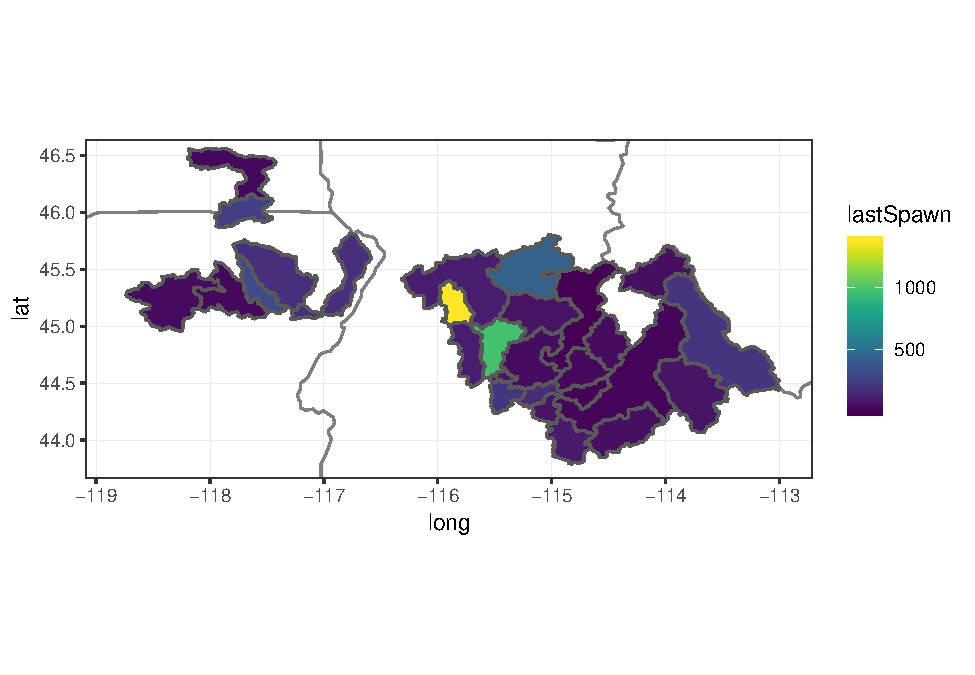
\includegraphics{4_Vis_IS_results_files/figure-latex/unnamed-chunk-5-1.pdf}

\begin{Shaded}
\begin{Highlighting}[]
\CommentTok{\# legend(x=.9, y=.8, legend = c("Ave Rank", "No. Models", "Highest Rank"), bty = "n", pch=20 , col=pal, text.col = "grey", cex=1, pt.cex=2)}


\CommentTok{\# par(op)}
\end{Highlighting}
\end{Shaded}

\hypertarget{b.-how-do-predator-interaction-strengths-compared-to-variables-from-other-domains-ocean-human}{%
\section{2b. How do predator interaction strengths compared to variables
from other domains (ocean,
human)?}\label{b.-how-do-predator-interaction-strengths-compared-to-variables-from-other-domains-ocean-human}}

\hypertarget{distribution-of-partial-derivatives-averaged-across-stocks-and-across-years-for-each-var}{%
\subsubsection{Distribution of partial derivatives, averaged across
stocks, and across years, for each
var}\label{distribution-of-partial-derivatives-averaged-across-stocks-and-across-years-for-each-var}}

\begin{Shaded}
\begin{Highlighting}[]
\NormalTok{rec4\_ESU }\OtherTok{\textless{}{-}}\NormalTok{  rec4\_ESU }\SpecialCharTok{\%\textgreater{}\%} 
  \FunctionTok{filter}\NormalTok{(}\SpecialCharTok{!}\FunctionTok{grepl}\NormalTok{(}\StringTok{"rec4"}\NormalTok{, FP)) }\SpecialCharTok{\%\textgreater{}\%} 
  \FunctionTok{group\_by}\NormalTok{(FP) }\SpecialCharTok{\%\textgreater{}\%} 
  \FunctionTok{mutate}\NormalTok{(}\AttributeTok{mu =} \FunctionTok{mean}\NormalTok{(value, }\AttributeTok{na.rm=}\ConstantTok{TRUE}\NormalTok{)) }\SpecialCharTok{\%\textgreater{}\%}
  \FunctionTok{ungroup}\NormalTok{()}

\FunctionTok{ggplot}\NormalTok{(rec4\_ESU, }\FunctionTok{aes}\NormalTok{(}\AttributeTok{x =}\NormalTok{ FP, }\AttributeTok{y =}\NormalTok{ value)) }\SpecialCharTok{+} 
  \FunctionTok{geom\_violin}\NormalTok{()}
\end{Highlighting}
\end{Shaded}

\includegraphics{4_Vis_IS_results_files/figure-latex/unnamed-chunk-6-1.pdf}

\begin{Shaded}
\begin{Highlighting}[]
\FunctionTok{ggplot}\NormalTok{(rec4\_ESU, }\FunctionTok{aes}\NormalTok{(}\AttributeTok{x =}\NormalTok{ value, }\AttributeTok{color =}\NormalTok{ FP, }\AttributeTok{fill =}\NormalTok{ FP)) }\SpecialCharTok{+}
  \FunctionTok{geom\_density}\NormalTok{(}\AttributeTok{alpha =} \FloatTok{0.4}\NormalTok{) }\SpecialCharTok{+}
  \FunctionTok{geom\_vline}\NormalTok{(}\FunctionTok{aes}\NormalTok{(}\AttributeTok{xintercept =}\NormalTok{ mu, }\AttributeTok{color =}\NormalTok{ FP),}
             \AttributeTok{linetype =} \StringTok{"dashed"}\NormalTok{)}
\end{Highlighting}
\end{Shaded}

\includegraphics{4_Vis_IS_results_files/figure-latex/unnamed-chunk-6-2.pdf}

\begin{Shaded}
\begin{Highlighting}[]
\CommentTok{\# Tough to see differences in this style}
\FunctionTok{unique}\NormalTok{(rec4\_ESU}\SpecialCharTok{$}\NormalTok{FP)}
\end{Highlighting}
\end{Shaded}

\begin{verbatim}
## [1] "npgo.win.3" "upw.tdmi.5" "pdo.spr.2"  "arc.win.2"
\end{verbatim}

\begin{Shaded}
\begin{Highlighting}[]
\NormalTok{rec4\_ESU}\SpecialCharTok{$}\NormalTok{FP }\OtherTok{=} \FunctionTok{factor}\NormalTok{(rec4\_ESU}\SpecialCharTok{$}\NormalTok{FP, }\AttributeTok{levels=}\FunctionTok{c}\NormalTok{(}\StringTok{\textquotesingle{}upw.tdmi.5\textquotesingle{}}\NormalTok{,}
                                                           \StringTok{\textquotesingle{}pdo.spr.2\textquotesingle{}}\NormalTok{,}
                                                           \StringTok{\textquotesingle{}arc.win.2\textquotesingle{}}\NormalTok{,}
                                                           \StringTok{\textquotesingle{}npgo.win.3\textquotesingle{}}\NormalTok{))}



\FunctionTok{ggplot}\NormalTok{(rec4\_ESU, }\FunctionTok{aes}\NormalTok{(}\AttributeTok{x =}\NormalTok{ value, }\AttributeTok{color =}\NormalTok{ FP, }\AttributeTok{fill =}\NormalTok{ FP)) }\SpecialCharTok{+}
  \FunctionTok{geom\_histogram}\NormalTok{(}\AttributeTok{position =} \StringTok{"identity"}\NormalTok{, }\AttributeTok{alpha =} \FloatTok{0.4}\NormalTok{) }\SpecialCharTok{+}
  \FunctionTok{scale\_color\_manual}\NormalTok{(}\AttributeTok{values =} \FunctionTok{colorRampPalette}\NormalTok{(}\FunctionTok{brewer.pal}\NormalTok{(}\DecValTok{9}\NormalTok{, }\StringTok{"Blues"}\NormalTok{))(}\DecValTok{8}\NormalTok{)[}\DecValTok{4}\SpecialCharTok{:}\DecValTok{7}\NormalTok{]) }\SpecialCharTok{+}
  \FunctionTok{scale\_fill\_manual}\NormalTok{(}\AttributeTok{values =} \FunctionTok{colorRampPalette}\NormalTok{(}\FunctionTok{brewer.pal}\NormalTok{(}\DecValTok{9}\NormalTok{, }\StringTok{"Blues"}\NormalTok{))(}\DecValTok{8}\NormalTok{)[}\DecValTok{4}\SpecialCharTok{:}\DecValTok{7}\NormalTok{]) }\SpecialCharTok{+}
    \FunctionTok{geom\_vline}\NormalTok{(}\FunctionTok{aes}\NormalTok{(}\AttributeTok{xintercept =}\NormalTok{ mu, }\AttributeTok{color =}\NormalTok{ FP),}
             \AttributeTok{linetype =} \StringTok{"dashed"}\NormalTok{)}\SpecialCharTok{+} 
  \FunctionTok{facet\_grid}\NormalTok{(FP }\SpecialCharTok{\textasciitilde{}}\NormalTok{ .)}
\end{Highlighting}
\end{Shaded}

\begin{verbatim}
## `stat_bin()` using `bins = 30`. Pick better value with `binwidth`.
\end{verbatim}

\includegraphics{4_Vis_IS_results_files/figure-latex/unnamed-chunk-6-3.pdf}

\begin{Shaded}
\begin{Highlighting}[]
\FunctionTok{ggplot}\NormalTok{(rec4\_ESU, }\FunctionTok{aes}\NormalTok{(}\AttributeTok{x =}\NormalTok{ value, }\AttributeTok{color =}\NormalTok{ FP, }\AttributeTok{fill =}\NormalTok{ FP)) }\SpecialCharTok{+}
  \FunctionTok{geom\_density}\NormalTok{(}\AttributeTok{alpha =} \FloatTok{0.4}\NormalTok{) }\SpecialCharTok{+}
  \FunctionTok{scale\_color\_manual}\NormalTok{(}\AttributeTok{values =} \FunctionTok{colorRampPalette}\NormalTok{(}\FunctionTok{brewer.pal}\NormalTok{(}\DecValTok{9}\NormalTok{, }\StringTok{"Blues"}\NormalTok{))(}\DecValTok{8}\NormalTok{)[}\DecValTok{4}\SpecialCharTok{:}\DecValTok{7}\NormalTok{]) }\SpecialCharTok{+}
  \FunctionTok{scale\_fill\_manual}\NormalTok{(}\AttributeTok{values =} \FunctionTok{colorRampPalette}\NormalTok{(}\FunctionTok{brewer.pal}\NormalTok{(}\DecValTok{9}\NormalTok{, }\StringTok{"Blues"}\NormalTok{))(}\DecValTok{8}\NormalTok{)[}\DecValTok{4}\SpecialCharTok{:}\DecValTok{7}\NormalTok{]) }\SpecialCharTok{+}
    \FunctionTok{geom\_vline}\NormalTok{(}\FunctionTok{aes}\NormalTok{(}\AttributeTok{xintercept =}\NormalTok{ mu, }\AttributeTok{color =}\NormalTok{ FP),}
             \AttributeTok{linetype =} \StringTok{"dashed"}\NormalTok{)}\SpecialCharTok{+} 
  \FunctionTok{facet\_grid}\NormalTok{(FP }\SpecialCharTok{\textasciitilde{}}\NormalTok{ .)}
\end{Highlighting}
\end{Shaded}

\includegraphics{4_Vis_IS_results_files/figure-latex/unnamed-chunk-6-4.pdf}

\hypertarget{how-do-predator-interaction-strengths-and-vars-from-other-domains-vary-through-time}{%
\section{3. How do predator interaction strengths (and vars from other
domains) vary through
time?}\label{how-do-predator-interaction-strengths-and-vars-from-other-domains-vary-through-time}}

\hypertarget{times-series-of-partial-derivatives-averaged-across-stocks-for-each-var}{%
\subsubsection{Times series of partial Derivatives, averaged across
stocks, for each
var}\label{times-series-of-partial-derivatives-averaged-across-stocks-for-each-var}}

\begin{Shaded}
\begin{Highlighting}[]
\FunctionTok{ggplot}\NormalTok{(rec4\_ESU, }\FunctionTok{aes}\NormalTok{(}\AttributeTok{x =}\NormalTok{ year, }\AttributeTok{y =}\NormalTok{ value, }\AttributeTok{fill =}\NormalTok{ FP, }\AttributeTok{color =}\NormalTok{ FP)) }\SpecialCharTok{+}
  \FunctionTok{geom\_smooth}\NormalTok{() }\SpecialCharTok{+}
  \FunctionTok{scale\_fill\_manual}\NormalTok{(}\AttributeTok{values =} \FunctionTok{colorRampPalette}\NormalTok{(}\FunctionTok{brewer.pal}\NormalTok{(}\DecValTok{9}\NormalTok{, }\StringTok{"Blues"}\NormalTok{))(}\DecValTok{8}\NormalTok{)[}\DecValTok{4}\SpecialCharTok{:}\DecValTok{7}\NormalTok{]) }\SpecialCharTok{+}
  \FunctionTok{scale\_color\_manual}\NormalTok{(}\AttributeTok{values =} \FunctionTok{colorRampPalette}\NormalTok{(}\FunctionTok{brewer.pal}\NormalTok{(}\DecValTok{9}\NormalTok{, }\StringTok{"Blues"}\NormalTok{))(}\DecValTok{8}\NormalTok{)[}\DecValTok{4}\SpecialCharTok{:}\DecValTok{7}\NormalTok{]) }\SpecialCharTok{+}
    \FunctionTok{geom\_hline}\NormalTok{(}\FunctionTok{aes}\NormalTok{(}\AttributeTok{yintercept =} \DecValTok{0}\NormalTok{),}
             \AttributeTok{linetype =} \StringTok{"dashed"}\NormalTok{) }\SpecialCharTok{+} 
  \FunctionTok{facet\_grid}\NormalTok{(FP }\SpecialCharTok{\textasciitilde{}}\NormalTok{ .)}
\end{Highlighting}
\end{Shaded}

\begin{verbatim}
## `geom_smooth()` using method = 'gam' and formula 'y ~ s(x, bs = "cs")'
\end{verbatim}

\includegraphics{4_Vis_IS_results_files/figure-latex/unnamed-chunk-7-1.pdf}

\begin{Shaded}
\begin{Highlighting}[]
\NormalTok{rec4\_ESU\_ts }\OtherTok{\textless{}{-}}\NormalTok{ rec4\_ESU }\SpecialCharTok{\%\textgreater{}\%} 
  \FunctionTok{filter}\NormalTok{(year }\SpecialCharTok{\textgreater{}} \DecValTok{1957}\NormalTok{) }\SpecialCharTok{\%\textgreater{}\%}
  \FunctionTok{filter}\NormalTok{(year }\SpecialCharTok{\textless{}} \DecValTok{2016}\NormalTok{) }\SpecialCharTok{\%\textgreater{}\%} 
  \FunctionTok{mutate}\NormalTok{(}\AttributeTok{year =} \FunctionTok{factor}\NormalTok{(year)) }\SpecialCharTok{\%\textgreater{}\%} 
  \FunctionTok{group\_by}\NormalTok{(year, FP) }\SpecialCharTok{\%\textgreater{}\%} 
  \FunctionTok{summarise}\NormalTok{(}\AttributeTok{IS =} \FunctionTok{mean}\NormalTok{(value, }\AttributeTok{na.rm =} \ConstantTok{TRUE}\NormalTok{), }
            \AttributeTok{sd =} \FunctionTok{sd}\NormalTok{(value, }\AttributeTok{na.rm =} \ConstantTok{TRUE}\NormalTok{),}
            \AttributeTok{n =} \FunctionTok{n}\NormalTok{()) }\SpecialCharTok{\%\textgreater{}\%}
  \FunctionTok{mutate}\NormalTok{(}\AttributeTok{se =}\NormalTok{ sd }\SpecialCharTok{/} \FunctionTok{sqrt}\NormalTok{(n),}
         \AttributeTok{lower =}\NormalTok{ IS }\SpecialCharTok{{-}} \FunctionTok{qt}\NormalTok{(}\DecValTok{1} \SpecialCharTok{{-}}\NormalTok{ (}\FloatTok{0.05} \SpecialCharTok{/} \DecValTok{2}\NormalTok{), n }\SpecialCharTok{{-}} \DecValTok{1}\NormalTok{) }\SpecialCharTok{*}\NormalTok{ se,}
         \AttributeTok{upper =}\NormalTok{ IS }\SpecialCharTok{+} \FunctionTok{qt}\NormalTok{(}\DecValTok{1} \SpecialCharTok{{-}}\NormalTok{ (}\FloatTok{0.05} \SpecialCharTok{/} \DecValTok{2}\NormalTok{), n }\SpecialCharTok{{-}} \DecValTok{1}\NormalTok{) }\SpecialCharTok{*}\NormalTok{ se) }\SpecialCharTok{\%\textgreater{}\%} 
  \FunctionTok{mutate}\NormalTok{(}\AttributeTok{year =} \FunctionTok{as.integer}\NormalTok{(year)) }\SpecialCharTok{\%\textgreater{}\%} 
\FunctionTok{ungroup}\NormalTok{() }\SpecialCharTok{\%\textgreater{}\%} \FunctionTok{ungroup}\NormalTok{() }
\end{Highlighting}
\end{Shaded}

\begin{verbatim}
## `summarise()` has grouped output by 'year'. You can override using the `.groups` argument.
\end{verbatim}

\begin{Shaded}
\begin{Highlighting}[]
\FunctionTok{ggplot}\NormalTok{(rec4\_ESU\_ts, }\FunctionTok{aes}\NormalTok{(}\AttributeTok{x =}\NormalTok{ year, }\AttributeTok{color =}\NormalTok{ FP, }\AttributeTok{fill =}\NormalTok{ FP)) }\SpecialCharTok{+}
  \FunctionTok{geom\_line}\NormalTok{(}\FunctionTok{aes}\NormalTok{(}\AttributeTok{y =}\NormalTok{ IS)) }\SpecialCharTok{+}
  \FunctionTok{geom\_line}\NormalTok{(}\FunctionTok{aes}\NormalTok{(}\AttributeTok{y =}\NormalTok{ upper), }\AttributeTok{alpha =} \FloatTok{0.5}\NormalTok{) }\SpecialCharTok{+}
  \FunctionTok{geom\_line}\NormalTok{(}\FunctionTok{aes}\NormalTok{(}\AttributeTok{y =}\NormalTok{ lower), }\AttributeTok{alpha =} \FloatTok{0.5}\NormalTok{) }\SpecialCharTok{+}
  \FunctionTok{geom\_hline}\NormalTok{(}\FunctionTok{aes}\NormalTok{(}\AttributeTok{yintercept =} \DecValTok{0}\NormalTok{),}
             \AttributeTok{linetype =} \StringTok{"dashed"}\NormalTok{) }\SpecialCharTok{+}
    \FunctionTok{scale\_fill\_manual}\NormalTok{(}\AttributeTok{values =} \FunctionTok{colorRampPalette}\NormalTok{(}\FunctionTok{brewer.pal}\NormalTok{(}\DecValTok{9}\NormalTok{, }\StringTok{"Blues"}\NormalTok{))(}\DecValTok{8}\NormalTok{)[}\DecValTok{4}\SpecialCharTok{:}\DecValTok{7}\NormalTok{]) }\SpecialCharTok{+}
  \FunctionTok{scale\_color\_manual}\NormalTok{(}\AttributeTok{values =} \FunctionTok{colorRampPalette}\NormalTok{(}\FunctionTok{brewer.pal}\NormalTok{(}\DecValTok{9}\NormalTok{, }\StringTok{"Blues"}\NormalTok{))(}\DecValTok{8}\NormalTok{)[}\DecValTok{4}\SpecialCharTok{:}\DecValTok{7}\NormalTok{]) }\SpecialCharTok{+}
     \FunctionTok{facet\_grid}\NormalTok{(FP }\SpecialCharTok{\textasciitilde{}}\NormalTok{ .)}
\end{Highlighting}
\end{Shaded}

\includegraphics{4_Vis_IS_results_files/figure-latex/unnamed-chunk-7-2.pdf}

\begin{Shaded}
\begin{Highlighting}[]
\NormalTok{rec4\_ESU\_lines }\OtherTok{\textless{}{-}}\NormalTok{ rec4\_ESU }\SpecialCharTok{\%\textgreater{}\%} 
  \FunctionTok{filter}\NormalTok{(year }\SpecialCharTok{\textgreater{}} \DecValTok{1957}\NormalTok{) }\SpecialCharTok{\%\textgreater{}\%}
  \FunctionTok{filter}\NormalTok{(year }\SpecialCharTok{\textless{}} \DecValTok{2016}\NormalTok{) }\SpecialCharTok{\%\textgreater{}\%} 
  \FunctionTok{mutate}\NormalTok{(}\AttributeTok{year =} \FunctionTok{factor}\NormalTok{(year)) }\SpecialCharTok{\%\textgreater{}\%} 
  \FunctionTok{group\_by}\NormalTok{(year, FP, embedding) }\SpecialCharTok{\%\textgreater{}\%} 
  \FunctionTok{mutate}\NormalTok{(}\AttributeTok{IS =} \FunctionTok{mean}\NormalTok{(value)) }\SpecialCharTok{\%\textgreater{}\%} 
  \FunctionTok{mutate}\NormalTok{(}\AttributeTok{year =} \FunctionTok{as.integer}\NormalTok{(year))}


\FunctionTok{ggplot}\NormalTok{() }\SpecialCharTok{+}
  \FunctionTok{geom\_line}\NormalTok{(rec4\_ESU\_lines, }\AttributeTok{mapping =} \FunctionTok{aes}\NormalTok{(}\AttributeTok{x=}\NormalTok{year, }\AttributeTok{y=}\NormalTok{IS, }\AttributeTok{col=}\NormalTok{FP, }\AttributeTok{group=}\NormalTok{embedding)) }\SpecialCharTok{+}    
  \FunctionTok{geom\_hline}\NormalTok{(rec4\_ESU\_lines, }\AttributeTok{mapping =} \FunctionTok{aes}\NormalTok{(}\AttributeTok{yintercept =} \DecValTok{0}\NormalTok{),}\AttributeTok{linetype =} \StringTok{"dashed"}\NormalTok{, }\AttributeTok{color =} \StringTok{"red"}\NormalTok{) }\SpecialCharTok{+}
  \FunctionTok{scale\_fill\_manual}\NormalTok{(}\AttributeTok{values =} \FunctionTok{colorRampPalette}\NormalTok{(}\FunctionTok{brewer.pal}\NormalTok{(}\DecValTok{9}\NormalTok{, }\StringTok{"Blues"}\NormalTok{))(}\DecValTok{8}\NormalTok{)[}\DecValTok{4}\SpecialCharTok{:}\DecValTok{7}\NormalTok{]) }\SpecialCharTok{+}
  \FunctionTok{scale\_color\_manual}\NormalTok{(}\AttributeTok{values =} \FunctionTok{colorRampPalette}\NormalTok{(}\FunctionTok{brewer.pal}\NormalTok{(}\DecValTok{9}\NormalTok{, }\StringTok{"Blues"}\NormalTok{))(}\DecValTok{8}\NormalTok{)[}\DecValTok{4}\SpecialCharTok{:}\DecValTok{7}\NormalTok{]) }\SpecialCharTok{+}
  \FunctionTok{geom\_line}\NormalTok{(rec4\_ESU\_ts, }\AttributeTok{mapping =} \FunctionTok{aes}\NormalTok{(}\AttributeTok{x=}\NormalTok{year, }\AttributeTok{y=}\NormalTok{IS), }\AttributeTok{color =} \StringTok{"black"}\NormalTok{) }\SpecialCharTok{+}
  \FunctionTok{facet\_grid}\NormalTok{(FP }\SpecialCharTok{\textasciitilde{}}\NormalTok{ ., }\AttributeTok{scales =} \StringTok{"free"}\NormalTok{) }\SpecialCharTok{+}
  \FunctionTok{theme\_bw}\NormalTok{()}
\end{Highlighting}
\end{Shaded}

\includegraphics{4_Vis_IS_results_files/figure-latex/unnamed-chunk-8-1.pdf}

\hypertarget{imn}{%
\section{IMN}\label{imn}}

\hypertarget{a.-what-variables-are-in-the-top-models-in-what-frequency-1}{%
\section{2a. What variables are in the top models? In what
frequency?}\label{a.-what-variables-are-in-the-top-models-in-what-frequency-1}}

\begin{Shaded}
\begin{Highlighting}[]
\FunctionTok{unique}\NormalTok{(rec4\_IMN}\SpecialCharTok{$}\NormalTok{FP)  }
\end{Highlighting}
\end{Shaded}

\begin{verbatim}
##  [1] "rec4n"             "rec4n_-3"          "flow.gageht.4"    
##  [4] "npgo.yrsum.3"      "pdo.spr.4"         "upw.tdmi.4"       
##  [7] "harv.COL.4"        "orca.SRKWpodJKL.4" "rec4n_-2"         
## [10] "rec4n_-5"          "rec4n_-4"          "rec4n_-1"         
## [13] "csl.males6.5"      "hatch.all.1"
\end{verbatim}

\begin{Shaded}
\begin{Highlighting}[]
\FunctionTok{unique}\NormalTok{(rec4\_IMN}\SpecialCharTok{$}\NormalTok{embedding)}\CommentTok{\# 54}
\end{Highlighting}
\end{Shaded}

\begin{verbatim}
##  [1]  1  2  3  4  5  6  7  8  9 10 11 12 13 14 15 16 17 18 19 20 21 22 23 24 25
## [26] 26 27 28 29 30 31 32 33 34 35 36 37 38 39 40 41 42 43 44 45 46 47 48 49 50
## [51] 51 52 53 54
\end{verbatim}

\begin{Shaded}
\begin{Highlighting}[]
\NormalTok{rec4\_mods }\OtherTok{\textless{}{-}}\NormalTok{ rec4\_IMN }\SpecialCharTok{\%\textgreater{}\%}
  \FunctionTok{group\_by}\NormalTok{(embedding, FP) }\SpecialCharTok{\%\textgreater{}\%} 
  \FunctionTok{summarise}\NormalTok{() }\SpecialCharTok{\%\textgreater{}\%} 
  \FunctionTok{group\_by}\NormalTok{(FP) }\SpecialCharTok{\%\textgreater{}\%} 
  \FunctionTok{mutate}\NormalTok{(}
    \AttributeTok{best\_mod =} \FunctionTok{min}\NormalTok{(embedding), }\CommentTok{\# lowest number (highest rank) model}
    \AttributeTok{scale\_mod =} \DecValTok{1} \SpecialCharTok{/}\NormalTok{ best\_mod, }\CommentTok{\# above expressed as 0{-}1}
    \AttributeTok{rank\_mod =} \FunctionTok{mean}\NormalTok{(embedding)}\SpecialCharTok{/}\DecValTok{54}\NormalTok{, }\CommentTok{\# average rank of model that that they are in}
    \AttributeTok{total\_num =} \FunctionTok{length}\NormalTok{(embedding), }\CommentTok{\# number of models that they are in}
    \AttributeTok{prop\_mod =}\NormalTok{ total\_num}\SpecialCharTok{/}\DecValTok{54}\NormalTok{, }\CommentTok{\# proportion of model that they are in }
    \AttributeTok{weight =} \DecValTok{54}\SpecialCharTok{{-}}\NormalTok{embedding, }\CommentTok{\# reverse of rank}
    \AttributeTok{integrated =} \FunctionTok{sum}\NormalTok{(weight)}\SpecialCharTok{/}\NormalTok{(}\DecValTok{54}\SpecialCharTok{*}\DecValTok{55}\SpecialCharTok{/}\DecValTok{2}\NormalTok{)) }\SpecialCharTok{\%\textgreater{}\%} \CommentTok{\# integrate rank and weight }
  \FunctionTok{slice}\NormalTok{(}\DecValTok{1}\NormalTok{) }\SpecialCharTok{\%\textgreater{}\%} 
  \FunctionTok{filter}\NormalTok{(}\SpecialCharTok{!}\FunctionTok{grepl}\NormalTok{(}\StringTok{"rec4"}\NormalTok{, FP)) }\SpecialCharTok{\%\textgreater{}\%} 
  \FunctionTok{filter}\NormalTok{(}\SpecialCharTok{!}\NormalTok{FP }\SpecialCharTok{==} \StringTok{"flow.gageht.4"}\NormalTok{) }\SpecialCharTok{\%\textgreater{}\%}
  \FunctionTok{ungroup}\NormalTok{()}
\end{Highlighting}
\end{Shaded}

\begin{verbatim}
## `summarise()` has grouped output by 'embedding'. You can override using the `.groups` argument.
\end{verbatim}

\begin{Shaded}
\begin{Highlighting}[]
\FunctionTok{unique}\NormalTok{(rec4\_mods}\SpecialCharTok{$}\NormalTok{FP)}
\end{Highlighting}
\end{Shaded}

\begin{verbatim}
## [1] "csl.males6.5"      "harv.COL.4"        "hatch.all.1"      
## [4] "npgo.yrsum.3"      "orca.SRKWpodJKL.4" "pdo.spr.4"        
## [7] "upw.tdmi.4"
\end{verbatim}

\begin{Shaded}
\begin{Highlighting}[]
\CommentTok{\# organize vars by Ocean, People, Biol}
\end{Highlighting}
\end{Shaded}

\begin{Shaded}
\begin{Highlighting}[]
\NormalTok{trans.pal }\OtherTok{\textless{}{-}} \FunctionTok{c}\NormalTok{(}\StringTok{"\#7BCAE44D"}\NormalTok{, }\StringTok{"\#E47BCA4D"}\NormalTok{, }\StringTok{"\#CAE47B4D"}\NormalTok{)}
\NormalTok{pal }\OtherTok{\textless{}{-}} \FunctionTok{c}\NormalTok{(}\StringTok{"\#7BCAE4"}\NormalTok{, }\StringTok{"\#E47BCA"}\NormalTok{, }\StringTok{"\#CAE47B"}\NormalTok{)}

\NormalTok{temp }\OtherTok{\textless{}{-}}\NormalTok{ rec4\_mods }\SpecialCharTok{\%\textgreater{}\%} 
  \FunctionTok{select}\NormalTok{(FP,prop\_mod, scale\_mod, rank\_mod) }\SpecialCharTok{\%\textgreater{}\%} 
  \FunctionTok{mutate}\NormalTok{(}\AttributeTok{ord =} \FunctionTok{c}\NormalTok{(}\DecValTok{1}\NormalTok{,}\DecValTok{5}\NormalTok{,}\DecValTok{6}\NormalTok{,}\DecValTok{2}\NormalTok{,}\DecValTok{7}\NormalTok{,}\DecValTok{3}\NormalTok{,}\DecValTok{4}\NormalTok{)) }\SpecialCharTok{\%\textgreater{}\%} 
  \FunctionTok{arrange}\NormalTok{(ord) }

\NormalTok{rec4\_spider }\OtherTok{\textless{}{-}} \FunctionTok{data.frame}\NormalTok{(}\FunctionTok{rbind}\NormalTok{(}\FunctionTok{rep}\NormalTok{(}\DecValTok{1}\NormalTok{,}\DecValTok{7}\NormalTok{), }\FunctionTok{rep}\NormalTok{(}\DecValTok{0}\NormalTok{,}\DecValTok{7}\NormalTok{), }
\NormalTok{                              temp}\SpecialCharTok{$}\NormalTok{rank\_mod, temp}\SpecialCharTok{$}\NormalTok{prop\_mod, temp}\SpecialCharTok{$}\NormalTok{scale\_mod }
\NormalTok{                                ))}
\FunctionTok{colnames}\NormalTok{(rec4\_spider) }\OtherTok{\textless{}{-}}\NormalTok{ temp}\SpecialCharTok{$}\NormalTok{FP}

\FunctionTok{radarchart}\NormalTok{(rec4\_spider, }\AttributeTok{axistype=}\DecValTok{0}\NormalTok{,}
           \CommentTok{\#custom polygon}
           \AttributeTok{pcol=}\NormalTok{pal, }\AttributeTok{pfcol=}\NormalTok{trans.pal,  }\AttributeTok{plwd=}\DecValTok{2}\NormalTok{, }\AttributeTok{plty=}\DecValTok{1}\NormalTok{, }\AttributeTok{seg =} \DecValTok{3}\NormalTok{,}
           \CommentTok{\#custom the grid}
           \AttributeTok{cglcol=}\StringTok{"grey"}\NormalTok{, }\AttributeTok{cglty=}\DecValTok{1}\NormalTok{, }\AttributeTok{cglwd=}\FloatTok{0.8}\NormalTok{,}
           \CommentTok{\#custom labels}
           \AttributeTok{vlcex=}\NormalTok{.}\DecValTok{9}\NormalTok{, }\AttributeTok{vlabels =} \FunctionTok{c}\NormalTok{(}\StringTok{"CSL"}\NormalTok{, }\StringTok{"NPGO"}\NormalTok{, }\StringTok{"PDO"}\NormalTok{, }\StringTok{"UPW"}\NormalTok{,  }\StringTok{"Harvest"}\NormalTok{,}
                                 \StringTok{"Hatchery"}\NormalTok{, }\StringTok{"ORCA"}\NormalTok{), }
           \AttributeTok{title=}\StringTok{"What variables are found in top models?"}\NormalTok{)}
\end{Highlighting}
\end{Shaded}

\includegraphics{4_Vis_IS_results_files/figure-latex/unnamed-chunk-10-1.pdf}

\hypertarget{b.-how-do-predator-interaction-strengths-compared-to-variables-from-other-domains-ocean-human-1}{%
\section{2b. How do predator interaction strengths compared to variables
from other domains (ocean,
human)?}\label{b.-how-do-predator-interaction-strengths-compared-to-variables-from-other-domains-ocean-human-1}}

\hypertarget{distribution-of-partial-derivatives-averaged-across-stocks-and-across-years-for-each-var-1}{%
\subsubsection{Distribution of partial derivatives, averaged across
stocks, and across years, for each
var}\label{distribution-of-partial-derivatives-averaged-across-stocks-and-across-years-for-each-var-1}}

\begin{Shaded}
\begin{Highlighting}[]
\NormalTok{rec4\_IMN}\OtherTok{\textless{}{-}}\NormalTok{  rec4\_IMN  }\SpecialCharTok{\%\textgreater{}\%} 
  \FunctionTok{filter}\NormalTok{(}\SpecialCharTok{!}\FunctionTok{grepl}\NormalTok{(}\StringTok{"rec4"}\NormalTok{, FP)) }\SpecialCharTok{\%\textgreater{}\%} 
  \FunctionTok{filter}\NormalTok{(}\SpecialCharTok{!}\FunctionTok{grepl}\NormalTok{(}\StringTok{"flow"}\NormalTok{, FP)) }\SpecialCharTok{\%\textgreater{}\%} 
  \FunctionTok{group\_by}\NormalTok{(FP) }\SpecialCharTok{\%\textgreater{}\%} 
  \FunctionTok{mutate}\NormalTok{(}\AttributeTok{mu =} \FunctionTok{mean}\NormalTok{(value, }\AttributeTok{na.rm=}\ConstantTok{TRUE}\NormalTok{)) }\SpecialCharTok{\%\textgreater{}\%}
  \FunctionTok{ungroup}\NormalTok{()}

\FunctionTok{ggplot}\NormalTok{(rec4\_IMN, }\FunctionTok{aes}\NormalTok{(}\AttributeTok{x =}\NormalTok{ FP, }\AttributeTok{y =}\NormalTok{ value)) }\SpecialCharTok{+} 
  \FunctionTok{geom\_violin}\NormalTok{()}
\end{Highlighting}
\end{Shaded}

\includegraphics{4_Vis_IS_results_files/figure-latex/unnamed-chunk-11-1.pdf}

\begin{Shaded}
\begin{Highlighting}[]
\NormalTok{rec4\_IMN}\SpecialCharTok{$}\NormalTok{domain }\OtherTok{=} \FunctionTok{factor}\NormalTok{(rec4\_IMN}\SpecialCharTok{$}\NormalTok{domain, }\AttributeTok{levels =} \FunctionTok{c}\NormalTok{( }\StringTok{"ocean"}\NormalTok{ , }\StringTok{"human"}\NormalTok{, }\StringTok{"pred"}\NormalTok{))}
\FunctionTok{unique}\NormalTok{(rec4\_IMN}\SpecialCharTok{$}\NormalTok{FP)}
\end{Highlighting}
\end{Shaded}

\begin{verbatim}
## [1] "npgo.yrsum.3"      "pdo.spr.4"         "upw.tdmi.4"       
## [4] "harv.COL.4"        "orca.SRKWpodJKL.4" "csl.males6.5"     
## [7] "hatch.all.1"
\end{verbatim}

\begin{Shaded}
\begin{Highlighting}[]
\NormalTok{rec4\_IMN}\SpecialCharTok{$}\NormalTok{FP }\OtherTok{=} \FunctionTok{factor}\NormalTok{(rec4\_IMN}\SpecialCharTok{$}\NormalTok{FP, }
                \AttributeTok{levels=}\FunctionTok{c}\NormalTok{(}\StringTok{\textquotesingle{}upw.tdmi.4\textquotesingle{}}\NormalTok{, }
                         \StringTok{\textquotesingle{}pdo.spr.4\textquotesingle{}}\NormalTok{,}
                         \StringTok{\textquotesingle{}npgo.yrsum.3\textquotesingle{}}\NormalTok{,}
                           \StringTok{\textquotesingle{}hatch.all.1\textquotesingle{}}\NormalTok{, }
                         \StringTok{"harv.COL.4"}\NormalTok{,}
                          \StringTok{"csl.males6.5"}\NormalTok{,}
                        \StringTok{"orca.SRKWpodJKL.4"}
                       
\NormalTok{                        ))}

\FunctionTok{ggplot}\NormalTok{(rec4\_IMN, }\FunctionTok{aes}\NormalTok{(}\AttributeTok{x =}\NormalTok{ value, }\AttributeTok{color =}\NormalTok{ domain, }\AttributeTok{fill =}\NormalTok{ domain)) }\SpecialCharTok{+}
  \FunctionTok{geom\_density}\NormalTok{(}\AttributeTok{alpha =} \FloatTok{0.4}\NormalTok{) }\SpecialCharTok{+}
  \FunctionTok{scale\_color\_manual}\NormalTok{(}\AttributeTok{values =}\NormalTok{ pal) }\SpecialCharTok{+}
  \FunctionTok{scale\_fill\_manual}\NormalTok{(}\AttributeTok{values =}\NormalTok{ pal) }\SpecialCharTok{+}
    \FunctionTok{geom\_vline}\NormalTok{(}\FunctionTok{aes}\NormalTok{(}\AttributeTok{xintercept =}\NormalTok{ mu, }\AttributeTok{color =}\NormalTok{ domain),}
             \AttributeTok{linetype =} \StringTok{"dashed"}\NormalTok{) }\SpecialCharTok{+} 
  \FunctionTok{facet\_grid}\NormalTok{(FP }\SpecialCharTok{\textasciitilde{}}\NormalTok{ .)}
\end{Highlighting}
\end{Shaded}

\includegraphics{4_Vis_IS_results_files/figure-latex/unnamed-chunk-11-2.pdf}

\hypertarget{how-do-predator-interaction-strengths-and-vars-from-other-domains-vary-through-time-1}{%
\section{3. How do predator interaction strengths (and vars from other
domains) vary through
time?}\label{how-do-predator-interaction-strengths-and-vars-from-other-domains-vary-through-time-1}}

\hypertarget{times-series-of-partial-derivatives-averaged-across-stocks-for-each-var-1}{%
\subsubsection{Times series of partial Derivatives, averaged across
stocks, for each
var}\label{times-series-of-partial-derivatives-averaged-across-stocks-for-each-var-1}}

\begin{Shaded}
\begin{Highlighting}[]
\FunctionTok{ggplot}\NormalTok{(rec4\_IMN, }\FunctionTok{aes}\NormalTok{(}\AttributeTok{x =}\NormalTok{ year, }\AttributeTok{y =}\NormalTok{ value, }\AttributeTok{fill =}\NormalTok{ domain, }\AttributeTok{color =}\NormalTok{ domain)) }\SpecialCharTok{+}
  \FunctionTok{geom\_smooth}\NormalTok{() }\SpecialCharTok{+}
  \FunctionTok{scale\_fill\_manual}\NormalTok{(}\AttributeTok{values =}\NormalTok{ pal) }\SpecialCharTok{+}
  \FunctionTok{scale\_color\_manual}\NormalTok{(}\AttributeTok{values =}\NormalTok{ pal) }\SpecialCharTok{+}
    \FunctionTok{geom\_hline}\NormalTok{(}\FunctionTok{aes}\NormalTok{(}\AttributeTok{yintercept =} \DecValTok{0}\NormalTok{),}
             \AttributeTok{linetype =} \StringTok{"dashed"}\NormalTok{) }\SpecialCharTok{+} 
  \FunctionTok{facet\_grid}\NormalTok{(FP }\SpecialCharTok{\textasciitilde{}}\NormalTok{ ., }\AttributeTok{scales =} \StringTok{"free"}\NormalTok{)}
\end{Highlighting}
\end{Shaded}

\begin{verbatim}
## `geom_smooth()` using method = 'gam' and formula 'y ~ s(x, bs = "cs")'
\end{verbatim}

\includegraphics{4_Vis_IS_results_files/figure-latex/unnamed-chunk-12-1.pdf}

\begin{Shaded}
\begin{Highlighting}[]
\NormalTok{rec4\_IMN\_ts }\OtherTok{\textless{}{-}}\NormalTok{ rec4\_IMN }\SpecialCharTok{\%\textgreater{}\%} 
  \FunctionTok{filter}\NormalTok{(year }\SpecialCharTok{\textgreater{}} \DecValTok{1957}\NormalTok{) }\SpecialCharTok{\%\textgreater{}\%}
  \FunctionTok{filter}\NormalTok{(year }\SpecialCharTok{\textless{}} \DecValTok{2016}\NormalTok{) }\SpecialCharTok{\%\textgreater{}\%} 
  \FunctionTok{mutate}\NormalTok{(}\AttributeTok{year =} \FunctionTok{factor}\NormalTok{(year)) }\SpecialCharTok{\%\textgreater{}\%} 
  \FunctionTok{group\_by}\NormalTok{(year, FP) }\SpecialCharTok{\%\textgreater{}\%} 
  \FunctionTok{mutate}\NormalTok{(}\AttributeTok{IS =} \FunctionTok{mean}\NormalTok{(value, }\AttributeTok{na.rm =} \ConstantTok{TRUE}\NormalTok{), }
            \AttributeTok{sd =} \FunctionTok{sd}\NormalTok{(value, }\AttributeTok{na.rm =} \ConstantTok{TRUE}\NormalTok{),}
            \AttributeTok{n =} \FunctionTok{n}\NormalTok{()) }\SpecialCharTok{\%\textgreater{}\%} 
  \FunctionTok{mutate}\NormalTok{(}\AttributeTok{se =}\NormalTok{ sd }\SpecialCharTok{/} \FunctionTok{sqrt}\NormalTok{(n),}
         \AttributeTok{lower =}\NormalTok{ IS }\SpecialCharTok{{-}} \FunctionTok{qt}\NormalTok{(}\DecValTok{1} \SpecialCharTok{{-}}\NormalTok{ (}\FloatTok{0.05} \SpecialCharTok{/} \DecValTok{2}\NormalTok{), n }\SpecialCharTok{{-}} \DecValTok{1}\NormalTok{) }\SpecialCharTok{*}\NormalTok{ se,}
         \AttributeTok{upper =}\NormalTok{ IS }\SpecialCharTok{+} \FunctionTok{qt}\NormalTok{(}\DecValTok{1} \SpecialCharTok{{-}}\NormalTok{ (}\FloatTok{0.05} \SpecialCharTok{/} \DecValTok{2}\NormalTok{), n }\SpecialCharTok{{-}} \DecValTok{1}\NormalTok{) }\SpecialCharTok{*}\NormalTok{ se) }\SpecialCharTok{\%\textgreater{}\%} 
  \FunctionTok{mutate}\NormalTok{(}\AttributeTok{year =} \FunctionTok{as.integer}\NormalTok{(year))}
\end{Highlighting}
\end{Shaded}

\begin{verbatim}
## Warning in qt(1 - (0.05/2), n - 1): NaNs produced

## Warning in qt(1 - (0.05/2), n - 1): NaNs produced

## Warning in qt(1 - (0.05/2), n - 1): NaNs produced

## Warning in qt(1 - (0.05/2), n - 1): NaNs produced
\end{verbatim}

\begin{Shaded}
\begin{Highlighting}[]
\FunctionTok{ggplot}\NormalTok{(rec4\_IMN\_ts, }\FunctionTok{aes}\NormalTok{(}\AttributeTok{x =}\NormalTok{ year, }\AttributeTok{color =}\NormalTok{ domain, }\AttributeTok{fill =}\NormalTok{ domain)) }\SpecialCharTok{+}
  \FunctionTok{geom\_line}\NormalTok{(}\FunctionTok{aes}\NormalTok{(}\AttributeTok{y =}\NormalTok{ IS)) }\SpecialCharTok{+}
  \FunctionTok{geom\_line}\NormalTok{(}\FunctionTok{aes}\NormalTok{(}\AttributeTok{y =}\NormalTok{ upper), }\AttributeTok{alpha =} \FloatTok{0.5}\NormalTok{) }\SpecialCharTok{+}
  \FunctionTok{geom\_line}\NormalTok{(}\FunctionTok{aes}\NormalTok{(}\AttributeTok{y =}\NormalTok{ lower), }\AttributeTok{alpha =} \FloatTok{0.5}\NormalTok{) }\SpecialCharTok{+}
  \FunctionTok{geom\_hline}\NormalTok{(}\FunctionTok{aes}\NormalTok{(}\AttributeTok{yintercept =} \DecValTok{0}\NormalTok{),}
             \AttributeTok{linetype =} \StringTok{"dashed"}\NormalTok{) }\SpecialCharTok{+}
    \FunctionTok{scale\_fill\_manual}\NormalTok{(}\AttributeTok{values =}\NormalTok{ pal) }\SpecialCharTok{+}
  \FunctionTok{scale\_color\_manual}\NormalTok{(}\AttributeTok{values =}\NormalTok{ pal) }\SpecialCharTok{+}
     \FunctionTok{facet\_wrap}\NormalTok{(}\SpecialCharTok{\textasciitilde{}}\NormalTok{ FP }\SpecialCharTok{+}\NormalTok{ domain, }\AttributeTok{scales =} \StringTok{"free"}\NormalTok{)}
\end{Highlighting}
\end{Shaded}

\includegraphics{4_Vis_IS_results_files/figure-latex/unnamed-chunk-13-1.pdf}

\begin{Shaded}
\begin{Highlighting}[]
\NormalTok{rec4\_IMN\_lines }\OtherTok{\textless{}{-}}\NormalTok{ rec4\_IMN }\SpecialCharTok{\%\textgreater{}\%} 
  \FunctionTok{filter}\NormalTok{(year }\SpecialCharTok{\textgreater{}} \DecValTok{1957}\NormalTok{) }\SpecialCharTok{\%\textgreater{}\%}
  \FunctionTok{filter}\NormalTok{(year }\SpecialCharTok{\textless{}} \DecValTok{2016}\NormalTok{) }\SpecialCharTok{\%\textgreater{}\%} 
  \FunctionTok{mutate}\NormalTok{(}\AttributeTok{year =} \FunctionTok{factor}\NormalTok{(year)) }\SpecialCharTok{\%\textgreater{}\%} 
  \FunctionTok{group\_by}\NormalTok{(year, FP, embedding) }\SpecialCharTok{\%\textgreater{}\%} 
  \FunctionTok{mutate}\NormalTok{(}\AttributeTok{IS =} \FunctionTok{mean}\NormalTok{(value)) }\SpecialCharTok{\%\textgreater{}\%} 
  \FunctionTok{mutate}\NormalTok{(}\AttributeTok{year =} \FunctionTok{as.integer}\NormalTok{(year))}


\FunctionTok{ggplot}\NormalTok{() }\SpecialCharTok{+}
  \FunctionTok{geom\_line}\NormalTok{(rec4\_IMN\_lines, }\AttributeTok{mapping =} \FunctionTok{aes}\NormalTok{(}\AttributeTok{x=}\NormalTok{year, }\AttributeTok{y=}\NormalTok{IS, }\AttributeTok{col=}\NormalTok{domain, }\AttributeTok{group=}\NormalTok{embedding)) }\SpecialCharTok{+} 
  \FunctionTok{scale\_fill\_manual}\NormalTok{(}\AttributeTok{values =}\NormalTok{ pal) }\SpecialCharTok{+}
  \FunctionTok{scale\_color\_manual}\NormalTok{(}\AttributeTok{values =}\NormalTok{ pal) }\SpecialCharTok{+}
  \FunctionTok{geom\_hline}\NormalTok{(rec4\_IMN\_lines, }\AttributeTok{mapping =} \FunctionTok{aes}\NormalTok{(}\AttributeTok{yintercept =} \DecValTok{0}\NormalTok{),}\AttributeTok{linetype =} \StringTok{"dashed"}\NormalTok{, }\AttributeTok{color =} \StringTok{"red"}\NormalTok{) }\SpecialCharTok{+}
  \FunctionTok{geom\_line}\NormalTok{(rec4\_IMN\_ts, }\AttributeTok{mapping =} \FunctionTok{aes}\NormalTok{(}\AttributeTok{x=}\NormalTok{year, }\AttributeTok{y=}\NormalTok{IS), }\AttributeTok{color =} \StringTok{"black"}\NormalTok{) }\SpecialCharTok{+}
  \FunctionTok{facet\_wrap}\NormalTok{(FP }\SpecialCharTok{+}\NormalTok{ domain }\SpecialCharTok{\textasciitilde{}}\NormalTok{ ., }\AttributeTok{scales =} \StringTok{"free"}\NormalTok{) }\SpecialCharTok{+}
  \FunctionTok{theme\_bw}\NormalTok{()}
\end{Highlighting}
\end{Shaded}

\includegraphics{4_Vis_IS_results_files/figure-latex/unnamed-chunk-14-1.pdf}

\hypertarget{mfs}{%
\section{MFS}\label{mfs}}

\begin{Shaded}
\begin{Highlighting}[]
\FunctionTok{unique}\NormalTok{(rec4\_MFS}\SpecialCharTok{$}\NormalTok{FP) }
\end{Highlighting}
\end{Shaded}

\begin{verbatim}
##  [1] "rec4n"          "rec4n_-1"       "rec4n_-4"       "arc.win.5"     
##  [5] "harv.CRsport.4" "pdo.sum.2"      "rec4n_-3"       "npgo.spr.3"    
##  [9] "rec4n_-2"       "upw.tdmi.4"     "hatch.SNAK.3"   "rec4n_-5"
\end{verbatim}

\begin{Shaded}
\begin{Highlighting}[]
\FunctionTok{unique}\NormalTok{(rec4\_MFS}\SpecialCharTok{$}\NormalTok{embedding)}
\end{Highlighting}
\end{Shaded}

\begin{verbatim}
##  [1]  1  2  3  4  5  6  7  8  9 10 11 12 13 14 15 16 17 18 19 20 21 22 23 24 25
## [26] 26 27 28 29 30 31 32 33 34 35 36 37 38 39 40 41 42 43 44
\end{verbatim}

\begin{Shaded}
\begin{Highlighting}[]
\NormalTok{rec4\_mods }\OtherTok{\textless{}{-}}\NormalTok{ rec4\_MFS }\SpecialCharTok{\%\textgreater{}\%}
  \FunctionTok{group\_by}\NormalTok{(embedding, FP) }\SpecialCharTok{\%\textgreater{}\%} 
  \FunctionTok{summarise}\NormalTok{() }\SpecialCharTok{\%\textgreater{}\%} 
  \FunctionTok{group\_by}\NormalTok{(FP) }\SpecialCharTok{\%\textgreater{}\%} 
  \FunctionTok{mutate}\NormalTok{(}
    \AttributeTok{best\_mod =} \FunctionTok{min}\NormalTok{(embedding), }\CommentTok{\# lowest number (highest rank) model}
    \AttributeTok{scale\_mod =} \DecValTok{1} \SpecialCharTok{/}\NormalTok{ best\_mod, }\CommentTok{\# above expressed as 0{-}1}
    \AttributeTok{rank\_mod =} \FunctionTok{mean}\NormalTok{(embedding)}\SpecialCharTok{/}\DecValTok{44}\NormalTok{, }\CommentTok{\# average rank of model that that they are in}
    \AttributeTok{total\_num =} \FunctionTok{length}\NormalTok{(embedding), }\CommentTok{\# number of models that they are in}
    \AttributeTok{prop\_mod =}\NormalTok{ total\_num}\SpecialCharTok{/}\DecValTok{44}\NormalTok{, }\CommentTok{\# proportion of model that they are in }
    \AttributeTok{weight =} \DecValTok{44}\SpecialCharTok{{-}}\NormalTok{embedding, }\CommentTok{\# reverse of rank}
    \AttributeTok{integrated =} \FunctionTok{sum}\NormalTok{(weight)}\SpecialCharTok{/}\NormalTok{(}\DecValTok{44}\SpecialCharTok{*}\DecValTok{45}\SpecialCharTok{/}\DecValTok{2}\NormalTok{)) }\SpecialCharTok{\%\textgreater{}\%} \CommentTok{\# integrate rank and weight }
  \FunctionTok{slice}\NormalTok{(}\DecValTok{1}\NormalTok{) }\SpecialCharTok{\%\textgreater{}\%} 
  \FunctionTok{filter}\NormalTok{(}\SpecialCharTok{!}\FunctionTok{grepl}\NormalTok{(}\StringTok{"rec4"}\NormalTok{, FP)) }\SpecialCharTok{\%\textgreater{}\%} 
  \FunctionTok{arrange}\NormalTok{(prop\_mod) }\SpecialCharTok{\%\textgreater{}\%} 
  \FunctionTok{ungroup}\NormalTok{()}
\end{Highlighting}
\end{Shaded}

\begin{verbatim}
## `summarise()` has grouped output by 'embedding'. You can override using the `.groups` argument.
\end{verbatim}

\begin{Shaded}
\begin{Highlighting}[]
\FunctionTok{unique}\NormalTok{(rec4\_mods}\SpecialCharTok{$}\NormalTok{FP)}
\end{Highlighting}
\end{Shaded}

\begin{verbatim}
## [1] "hatch.SNAK.3"   "npgo.spr.3"     "upw.tdmi.4"     "pdo.sum.2"     
## [5] "arc.win.5"      "harv.CRsport.4"
\end{verbatim}

\begin{Shaded}
\begin{Highlighting}[]
\NormalTok{temp }\OtherTok{\textless{}{-}}\NormalTok{ rec4\_mods }\SpecialCharTok{\%\textgreater{}\%} 
  \FunctionTok{select}\NormalTok{(FP, prop\_mod, scale\_mod, rank\_mod) }\SpecialCharTok{\%\textgreater{}\%} 
  \FunctionTok{mutate}\NormalTok{(}\AttributeTok{ord =} \FunctionTok{c}\NormalTok{(}\DecValTok{1}\NormalTok{,}\DecValTok{2}\NormalTok{,}\DecValTok{4}\NormalTok{,}\DecValTok{3}\NormalTok{,}\DecValTok{5}\NormalTok{,}\DecValTok{6}\NormalTok{)) }\SpecialCharTok{\%\textgreater{}\%} 
  \FunctionTok{arrange}\NormalTok{(ord) }

\NormalTok{rec4\_spider }\OtherTok{\textless{}{-}} \FunctionTok{data.frame}\NormalTok{(}\FunctionTok{rbind}\NormalTok{(}\FunctionTok{rep}\NormalTok{(}\DecValTok{1}\NormalTok{,}\DecValTok{6}\NormalTok{), }\FunctionTok{rep}\NormalTok{(}\DecValTok{0}\NormalTok{,}\DecValTok{6}\NormalTok{), }
\NormalTok{                              temp}\SpecialCharTok{$}\NormalTok{rank\_mod, temp}\SpecialCharTok{$}\NormalTok{prop\_mod, temp}\SpecialCharTok{$}\NormalTok{scale\_mod }
\NormalTok{                                ))}
\FunctionTok{colnames}\NormalTok{(rec4\_spider) }\OtherTok{\textless{}{-}}\NormalTok{ temp}\SpecialCharTok{$}\NormalTok{FP}

\NormalTok{trans.pal }\OtherTok{\textless{}{-}} \FunctionTok{c}\NormalTok{(}\StringTok{"\#7BCAE44D"}\NormalTok{, }\StringTok{"\#E47BCA4D"}\NormalTok{, }\StringTok{"\#CAE47B4D"}\NormalTok{)}
\NormalTok{pal }\OtherTok{\textless{}{-}} \FunctionTok{c}\NormalTok{(}\StringTok{"\#7BCAE4"}\NormalTok{, }\StringTok{"\#E47BCA"}\NormalTok{, }\StringTok{"\#CAE47B"}\NormalTok{)}

\CommentTok{\# op \textless{}{-} par(mar = c(1, 1, 1, 1))}
\CommentTok{\# par(mar = c(1, 0, 1, 5))}

\FunctionTok{radarchart}\NormalTok{(rec4\_spider, }\AttributeTok{axistype=}\DecValTok{0}\NormalTok{,}
           \CommentTok{\#custom polygon}
           \AttributeTok{pcol=}\NormalTok{pal, }\AttributeTok{pfcol=}\NormalTok{trans.pal,  }\AttributeTok{plwd=}\DecValTok{2}\NormalTok{, }\AttributeTok{plty=}\DecValTok{1}\NormalTok{, }\AttributeTok{seg =} \DecValTok{3}\NormalTok{,}
           \CommentTok{\#custom the grid}
           \AttributeTok{cglcol=}\StringTok{"grey"}\NormalTok{, }\AttributeTok{cglty=}\DecValTok{1}\NormalTok{, }\AttributeTok{cglwd=}\FloatTok{0.8}\NormalTok{,}
           \CommentTok{\#custom labels}
           \AttributeTok{vlcex=}\NormalTok{.}\DecValTok{9}\NormalTok{, }\AttributeTok{vlabels =} \FunctionTok{c}\NormalTok{(}\StringTok{"Hatchery"}\NormalTok{, }\StringTok{"NPGO"}\NormalTok{, }\StringTok{"PDO"}\NormalTok{, }\StringTok{"UPW"}\NormalTok{, }\StringTok{"ARC"}\NormalTok{, }\StringTok{"Harvest"}\NormalTok{), }
           \AttributeTok{title=}\StringTok{"What variables are found in top models?"}\NormalTok{)}
\end{Highlighting}
\end{Shaded}

\includegraphics{4_Vis_IS_results_files/figure-latex/unnamed-chunk-16-1.pdf}

\begin{Shaded}
\begin{Highlighting}[]
\CommentTok{\# legend(x=.9, y=.8, legend = c("Ave Rank", "No. Models", "Highest Rank"), bty = "n", pch=20 , col=pal, text.col = "grey", cex=1, pt.cex=2)}


\CommentTok{\# par(op)}
\end{Highlighting}
\end{Shaded}

\hypertarget{b.-how-do-predator-interaction-strengths-compared-to-variables-from-other-domains-ocean-human-2}{%
\section{2b. How do predator interaction strengths compared to variables
from other domains (ocean,
human)?}\label{b.-how-do-predator-interaction-strengths-compared-to-variables-from-other-domains-ocean-human-2}}

\hypertarget{partial-derivatives-averaged-across-stocks-and-across-years-for-each}{%
\subsubsection{Partial Derivatives, averaged across stocks, and across
years, for
each}\label{partial-derivatives-averaged-across-stocks-and-across-years-for-each}}

\begin{Shaded}
\begin{Highlighting}[]
\NormalTok{rec4\_MFS}\OtherTok{\textless{}{-}}\NormalTok{  rec4\_MFS  }\SpecialCharTok{\%\textgreater{}\%} 
  \FunctionTok{filter}\NormalTok{(}\SpecialCharTok{!}\FunctionTok{grepl}\NormalTok{(}\StringTok{"rec4"}\NormalTok{, FP)) }\SpecialCharTok{\%\textgreater{}\%} 
  \FunctionTok{filter}\NormalTok{(}\SpecialCharTok{!}\FunctionTok{grepl}\NormalTok{(}\StringTok{"flow"}\NormalTok{, FP)) }\SpecialCharTok{\%\textgreater{}\%} 
  \FunctionTok{group\_by}\NormalTok{(FP) }\SpecialCharTok{\%\textgreater{}\%} 
  \FunctionTok{mutate}\NormalTok{(}\AttributeTok{mu =} \FunctionTok{mean}\NormalTok{(value, }\AttributeTok{na.rm=}\ConstantTok{TRUE}\NormalTok{)) }\SpecialCharTok{\%\textgreater{}\%}
  \FunctionTok{ungroup}\NormalTok{()}

\FunctionTok{ggplot}\NormalTok{(rec4\_MFS, }\FunctionTok{aes}\NormalTok{(}\AttributeTok{x =}\NormalTok{ FP, }\AttributeTok{y =}\NormalTok{ value)) }\SpecialCharTok{+} 
  \FunctionTok{geom\_violin}\NormalTok{()}
\end{Highlighting}
\end{Shaded}

\includegraphics{4_Vis_IS_results_files/figure-latex/unnamed-chunk-17-1.pdf}

\begin{Shaded}
\begin{Highlighting}[]
\NormalTok{rec4\_MFS}\SpecialCharTok{$}\NormalTok{domain }\OtherTok{=} \FunctionTok{factor}\NormalTok{(rec4\_MFS}\SpecialCharTok{$}\NormalTok{domain, }\AttributeTok{levels =} \FunctionTok{c}\NormalTok{( }\StringTok{"ocean"}\NormalTok{, }\StringTok{"pred"}\NormalTok{, }\StringTok{"human"}\NormalTok{))}
\FunctionTok{unique}\NormalTok{(rec4\_MFS}\SpecialCharTok{$}\NormalTok{FP) }
\end{Highlighting}
\end{Shaded}

\begin{verbatim}
## [1] "arc.win.5"      "harv.CRsport.4" "pdo.sum.2"      "npgo.spr.3"    
## [5] "upw.tdmi.4"     "hatch.SNAK.3"
\end{verbatim}

\begin{Shaded}
\begin{Highlighting}[]
\NormalTok{rec4\_MFS}\SpecialCharTok{$}\NormalTok{FP }\OtherTok{=} \FunctionTok{factor}\NormalTok{(rec4\_MFS}\SpecialCharTok{$}\NormalTok{FP, }
                \AttributeTok{levels=}\FunctionTok{c}\NormalTok{(}\StringTok{\textquotesingle{}arc.win.5\textquotesingle{}}\NormalTok{,}
                         \StringTok{\textquotesingle{}upw.tdmi.4\textquotesingle{}}\NormalTok{, }
                         \StringTok{\textquotesingle{}pdo.sum.2\textquotesingle{}}\NormalTok{,}
                         \StringTok{\textquotesingle{}npgo.spr.3\textquotesingle{}}\NormalTok{,}
                         \StringTok{\textquotesingle{}hatch.SNAK.3\textquotesingle{}}\NormalTok{, }
                         \StringTok{"harv.CRsport.4"}
\NormalTok{                        ))}

\FunctionTok{ggplot}\NormalTok{(rec4\_MFS, }\FunctionTok{aes}\NormalTok{(}\AttributeTok{x =}\NormalTok{ year, }\AttributeTok{y =}\NormalTok{ value, }\AttributeTok{fill =}\NormalTok{ domain, }\AttributeTok{color =}\NormalTok{ domain)) }\SpecialCharTok{+}
  \FunctionTok{geom\_smooth}\NormalTok{() }\SpecialCharTok{+}
  \FunctionTok{scale\_fill\_manual}\NormalTok{(}\AttributeTok{values =}\NormalTok{ pal) }\SpecialCharTok{+}
  \FunctionTok{scale\_color\_manual}\NormalTok{(}\AttributeTok{values =}\NormalTok{ pal) }\SpecialCharTok{+}
    \FunctionTok{geom\_hline}\NormalTok{(}\FunctionTok{aes}\NormalTok{(}\AttributeTok{yintercept =} \DecValTok{0}\NormalTok{),}
             \AttributeTok{linetype =} \StringTok{"dashed"}\NormalTok{) }\SpecialCharTok{+} 
  \FunctionTok{facet\_grid}\NormalTok{(FP }\SpecialCharTok{\textasciitilde{}}\NormalTok{ ., }\AttributeTok{scales =} \StringTok{"free"}\NormalTok{)}
\end{Highlighting}
\end{Shaded}

\begin{verbatim}
## `geom_smooth()` using method = 'gam' and formula 'y ~ s(x, bs = "cs")'
\end{verbatim}

\includegraphics{4_Vis_IS_results_files/figure-latex/unnamed-chunk-17-2.pdf}

\begin{Shaded}
\begin{Highlighting}[]
\CommentTok{\# distribution}

\FunctionTok{ggplot}\NormalTok{(rec4\_MFS, }\FunctionTok{aes}\NormalTok{(}\AttributeTok{x =}\NormalTok{ value, }\AttributeTok{color =}\NormalTok{ domain, }\AttributeTok{fill =}\NormalTok{ domain)) }\SpecialCharTok{+}
  \FunctionTok{geom\_density}\NormalTok{(}\AttributeTok{alpha =} \FloatTok{0.4}\NormalTok{) }\SpecialCharTok{+}
  \FunctionTok{scale\_color\_manual}\NormalTok{(}\AttributeTok{values =}\NormalTok{ pal) }\SpecialCharTok{+}
  \FunctionTok{scale\_fill\_manual}\NormalTok{(}\AttributeTok{values =}\NormalTok{ pal) }\SpecialCharTok{+}
    \FunctionTok{geom\_vline}\NormalTok{(}\FunctionTok{aes}\NormalTok{(}\AttributeTok{xintercept =}\NormalTok{ mu, }\AttributeTok{color =}\NormalTok{ domain),}
             \AttributeTok{linetype =} \StringTok{"dashed"}\NormalTok{) }\SpecialCharTok{+} 
  \FunctionTok{facet\_grid}\NormalTok{(FP }\SpecialCharTok{\textasciitilde{}}\NormalTok{ .)}
\end{Highlighting}
\end{Shaded}

\includegraphics{4_Vis_IS_results_files/figure-latex/unnamed-chunk-17-3.pdf}
\# 3. How do predator interaction strengths (and vars from other
domains) vary through time? \#\#\# Times series of partial Derivatives,
averaged across stocks, for each var

\begin{Shaded}
\begin{Highlighting}[]
\NormalTok{rec4\_MFS\_ts }\OtherTok{\textless{}{-}}\NormalTok{ rec4\_MFS }\SpecialCharTok{\%\textgreater{}\%} 
  \FunctionTok{filter}\NormalTok{(year }\SpecialCharTok{\textgreater{}} \DecValTok{1957}\NormalTok{) }\SpecialCharTok{\%\textgreater{}\%}
  \FunctionTok{filter}\NormalTok{(year }\SpecialCharTok{\textless{}} \DecValTok{2016}\NormalTok{) }\SpecialCharTok{\%\textgreater{}\%} 
  \FunctionTok{mutate}\NormalTok{(}\AttributeTok{year =} \FunctionTok{factor}\NormalTok{(year)) }\SpecialCharTok{\%\textgreater{}\%} 
  \FunctionTok{group\_by}\NormalTok{(year, FP) }\SpecialCharTok{\%\textgreater{}\%} 
  \FunctionTok{mutate}\NormalTok{(}\AttributeTok{IS =} \FunctionTok{mean}\NormalTok{(value, }\AttributeTok{na.rm =} \ConstantTok{TRUE}\NormalTok{), }
            \AttributeTok{sd =} \FunctionTok{sd}\NormalTok{(value, }\AttributeTok{na.rm =} \ConstantTok{TRUE}\NormalTok{),}
            \AttributeTok{n =} \FunctionTok{n}\NormalTok{()) }\SpecialCharTok{\%\textgreater{}\%} 
  \FunctionTok{mutate}\NormalTok{(}\AttributeTok{se =}\NormalTok{ sd }\SpecialCharTok{/} \FunctionTok{sqrt}\NormalTok{(n),}
         \AttributeTok{lower =}\NormalTok{ IS }\SpecialCharTok{{-}} \FunctionTok{qt}\NormalTok{(}\DecValTok{1} \SpecialCharTok{{-}}\NormalTok{ (}\FloatTok{0.05} \SpecialCharTok{/} \DecValTok{2}\NormalTok{), n }\SpecialCharTok{{-}} \DecValTok{1}\NormalTok{) }\SpecialCharTok{*}\NormalTok{ se,}
         \AttributeTok{upper =}\NormalTok{ IS }\SpecialCharTok{+} \FunctionTok{qt}\NormalTok{(}\DecValTok{1} \SpecialCharTok{{-}}\NormalTok{ (}\FloatTok{0.05} \SpecialCharTok{/} \DecValTok{2}\NormalTok{), n }\SpecialCharTok{{-}} \DecValTok{1}\NormalTok{) }\SpecialCharTok{*}\NormalTok{ se) }\SpecialCharTok{\%\textgreater{}\%} 
  \FunctionTok{mutate}\NormalTok{(}\AttributeTok{year =} \FunctionTok{as.integer}\NormalTok{(year))}
  
\FunctionTok{ggplot}\NormalTok{(rec4\_MFS\_ts, }\FunctionTok{aes}\NormalTok{(}\AttributeTok{x =}\NormalTok{ year, }\AttributeTok{color =}\NormalTok{ domain, }\AttributeTok{fill =}\NormalTok{ domain)) }\SpecialCharTok{+}
  \FunctionTok{geom\_line}\NormalTok{(}\FunctionTok{aes}\NormalTok{(}\AttributeTok{y =}\NormalTok{ IS)) }\SpecialCharTok{+}
  \FunctionTok{geom\_line}\NormalTok{(}\FunctionTok{aes}\NormalTok{(}\AttributeTok{y =}\NormalTok{ upper), }\AttributeTok{alpha =} \FloatTok{0.5}\NormalTok{) }\SpecialCharTok{+}
  \FunctionTok{geom\_line}\NormalTok{(}\FunctionTok{aes}\NormalTok{(}\AttributeTok{y =}\NormalTok{ lower), }\AttributeTok{alpha =} \FloatTok{0.5}\NormalTok{) }\SpecialCharTok{+}
  \FunctionTok{geom\_hline}\NormalTok{(}\FunctionTok{aes}\NormalTok{(}\AttributeTok{yintercept =} \DecValTok{0}\NormalTok{),}
             \AttributeTok{linetype =} \StringTok{"dashed"}\NormalTok{) }\SpecialCharTok{+}
    \FunctionTok{scale\_fill\_manual}\NormalTok{(}\AttributeTok{values =}\NormalTok{ pal) }\SpecialCharTok{+}
  \FunctionTok{scale\_color\_manual}\NormalTok{(}\AttributeTok{values =}\NormalTok{ pal) }\SpecialCharTok{+}
     \FunctionTok{facet\_wrap}\NormalTok{(}\SpecialCharTok{\textasciitilde{}}\NormalTok{ FP }\SpecialCharTok{+}\NormalTok{ domain, }\AttributeTok{scales =} \StringTok{"free"}\NormalTok{)}
\end{Highlighting}
\end{Shaded}

\includegraphics{4_Vis_IS_results_files/figure-latex/unnamed-chunk-18-1.pdf}

\begin{Shaded}
\begin{Highlighting}[]
\NormalTok{rec4\_MFS\_lines }\OtherTok{\textless{}{-}}\NormalTok{ rec4\_MFS }\SpecialCharTok{\%\textgreater{}\%} 
  \FunctionTok{filter}\NormalTok{(year }\SpecialCharTok{\textgreater{}} \DecValTok{1957}\NormalTok{) }\SpecialCharTok{\%\textgreater{}\%}
  \FunctionTok{filter}\NormalTok{(year }\SpecialCharTok{\textless{}} \DecValTok{2016}\NormalTok{) }\SpecialCharTok{\%\textgreater{}\%} 
  \FunctionTok{mutate}\NormalTok{(}\AttributeTok{year =} \FunctionTok{factor}\NormalTok{(year)) }\SpecialCharTok{\%\textgreater{}\%} 
  \FunctionTok{group\_by}\NormalTok{(year, FP, embedding) }\SpecialCharTok{\%\textgreater{}\%} 
  \FunctionTok{mutate}\NormalTok{(}\AttributeTok{IS =} \FunctionTok{mean}\NormalTok{(value)) }\SpecialCharTok{\%\textgreater{}\%} 
  \FunctionTok{mutate}\NormalTok{(}\AttributeTok{year =} \FunctionTok{as.integer}\NormalTok{(year))}


\FunctionTok{ggplot}\NormalTok{() }\SpecialCharTok{+}
  \FunctionTok{geom\_line}\NormalTok{(rec4\_MFS\_lines, }\AttributeTok{mapping =} \FunctionTok{aes}\NormalTok{(}\AttributeTok{x=}\NormalTok{year, }\AttributeTok{y=}\NormalTok{IS, }\AttributeTok{col=}\NormalTok{domain, }\AttributeTok{group=}\NormalTok{embedding)) }\SpecialCharTok{+} 
  \FunctionTok{scale\_fill\_manual}\NormalTok{(}\AttributeTok{values =}\NormalTok{ pal) }\SpecialCharTok{+}
  \FunctionTok{scale\_color\_manual}\NormalTok{(}\AttributeTok{values =}\NormalTok{ pal) }\SpecialCharTok{+}
  \FunctionTok{geom\_hline}\NormalTok{(rec4\_MFS\_lines, }\AttributeTok{mapping =} \FunctionTok{aes}\NormalTok{(}\AttributeTok{yintercept =} \DecValTok{0}\NormalTok{),}\AttributeTok{linetype =} \StringTok{"dashed"}\NormalTok{, }\AttributeTok{color =} \StringTok{"red"}\NormalTok{) }\SpecialCharTok{+}
  \FunctionTok{geom\_line}\NormalTok{(rec4\_MFS\_ts, }\AttributeTok{mapping =} \FunctionTok{aes}\NormalTok{(}\AttributeTok{x=}\NormalTok{year, }\AttributeTok{y=}\NormalTok{IS), }\AttributeTok{color =} \StringTok{"black"}\NormalTok{) }\SpecialCharTok{+}
  \FunctionTok{facet\_wrap}\NormalTok{(FP }\SpecialCharTok{+}\NormalTok{ domain }\SpecialCharTok{\textasciitilde{}}\NormalTok{ ., }\AttributeTok{scales =} \StringTok{"free"}\NormalTok{) }\SpecialCharTok{+}
  \FunctionTok{theme\_bw}\NormalTok{()}
\end{Highlighting}
\end{Shaded}

\includegraphics{4_Vis_IS_results_files/figure-latex/unnamed-chunk-19-1.pdf}

\hypertarget{ups}{%
\section{UPS}\label{ups}}

\hypertarget{a.-what-variables-are-in-the-top-models-in-what-frequency-2}{%
\section{2a. What variables are in the top models? In what
frequency?}\label{a.-what-variables-are-in-the-top-models-in-what-frequency-2}}

\hypertarget{to-do-that-right-we-need-to-actually-through-all-the-vars-in-the-smap-hopper-not-just-the-top-ones-1}{%
\subsubsection{To do that right, we need to actually through ALL the
vars in the SMAP hopper, not just the top
ones}\label{to-do-that-right-we-need-to-actually-through-all-the-vars-in-the-smap-hopper-not-just-the-top-ones-1}}

\hypertarget{but-i-can-get-an-highest-and-average-rank-model-that-each-var-shows-up-in-1}{%
\subsubsection{But I can get an highest and average rank model that each
var shows up
in}\label{but-i-can-get-an-highest-and-average-rank-model-that-each-var-shows-up-in-1}}

\begin{Shaded}
\begin{Highlighting}[]
\FunctionTok{unique}\NormalTok{(rec4\_UPS}\SpecialCharTok{$}\NormalTok{FP)     }
\end{Highlighting}
\end{Shaded}

\begin{verbatim}
##  [1] "rec4n"                "rec4n_-1"             "harv.PACtot.5"       
##  [4] "hseal.COL.3"          "hatch.total.1"        "pdo.sum.5"           
##  [7] "ssl.COL.4"            "orca.SRKWdeathsJKL.5" "rec4n_-3"            
## [10] "csl.Dpups.0"          "npgo.spr.2"           "upw.tdmi.5"          
## [13] "rec4n_-2"             "flow.mean.1"
\end{verbatim}

\begin{Shaded}
\begin{Highlighting}[]
\NormalTok{rec4\_mods }\OtherTok{\textless{}{-}}\NormalTok{ rec4\_UPS }\SpecialCharTok{\%\textgreater{}\%}
  \FunctionTok{group\_by}\NormalTok{(embedding, FP) }\SpecialCharTok{\%\textgreater{}\%} 
  \FunctionTok{summarise}\NormalTok{() }\SpecialCharTok{\%\textgreater{}\%} 
  \FunctionTok{group\_by}\NormalTok{(FP) }\SpecialCharTok{\%\textgreater{}\%} 
  \FunctionTok{mutate}\NormalTok{(}
    \AttributeTok{best\_mod =} \FunctionTok{min}\NormalTok{(embedding), }\CommentTok{\# lowest number (highest rank) model}
    \AttributeTok{scale\_mod =} \DecValTok{1} \SpecialCharTok{/}\NormalTok{ best\_mod, }\CommentTok{\# above expressed as 0{-}1}
    \AttributeTok{rank\_mod =} \FunctionTok{mean}\NormalTok{(embedding)}\SpecialCharTok{/}\DecValTok{16}\NormalTok{, }\CommentTok{\# average rank of model that that they are in}
    \AttributeTok{total\_num =} \FunctionTok{length}\NormalTok{(embedding), }\CommentTok{\# number of models that they are in}
    \AttributeTok{prop\_mod =}\NormalTok{ total\_num}\SpecialCharTok{/}\DecValTok{12}\NormalTok{, }\CommentTok{\# proportion of model that they are in }
    \AttributeTok{weight =} \DecValTok{17}\SpecialCharTok{{-}}\NormalTok{embedding, }\CommentTok{\# reverse of rank}
    \AttributeTok{integrated =} \FunctionTok{sum}\NormalTok{(weight)}\SpecialCharTok{/}\NormalTok{(}\DecValTok{16}\SpecialCharTok{*}\DecValTok{17}\SpecialCharTok{/}\DecValTok{2}\NormalTok{)) }\SpecialCharTok{\%\textgreater{}\%} \CommentTok{\# integrate rank and weight }
  \FunctionTok{slice}\NormalTok{(}\DecValTok{1}\NormalTok{) }\SpecialCharTok{\%\textgreater{}\%} 
  \FunctionTok{filter}\NormalTok{(}\SpecialCharTok{!}\FunctionTok{grepl}\NormalTok{(}\StringTok{"rec4"}\NormalTok{, FP)) }\SpecialCharTok{\%\textgreater{}\%} 
  \FunctionTok{arrange}\NormalTok{(prop\_mod) }\SpecialCharTok{\%\textgreater{}\%} 
  \FunctionTok{filter}\NormalTok{(}\SpecialCharTok{!}\NormalTok{FP }\SpecialCharTok{==} \StringTok{"flow.mean.1"}\NormalTok{) }\SpecialCharTok{\%\textgreater{}\%} 
  \FunctionTok{filter}\NormalTok{(}\SpecialCharTok{!}\NormalTok{FP }\SpecialCharTok{==} \StringTok{"hseal.COL.3"}\NormalTok{) }\SpecialCharTok{\%\textgreater{}\%}
  \FunctionTok{ungroup}\NormalTok{()}
\end{Highlighting}
\end{Shaded}

\begin{verbatim}
## `summarise()` has grouped output by 'embedding'. You can override using the `.groups` argument.
\end{verbatim}

\begin{Shaded}
\begin{Highlighting}[]
\NormalTok{rec4\_mods}\SpecialCharTok{$}\NormalTok{FP }\OtherTok{\textless{}{-}} \FunctionTok{factor}\NormalTok{(rec4\_mods}\SpecialCharTok{$}\NormalTok{FP, }\AttributeTok{levels =} \FunctionTok{c}\NormalTok{(}\StringTok{"npgo.spr.2"}\NormalTok{, }
                                                \StringTok{"pdo.sum.5"}\NormalTok{, }
                                                \StringTok{"upw.tdmi.5"}\NormalTok{,}
                                                \StringTok{"harv.PACtot.5"}\NormalTok{,}
                                                \StringTok{"hatch.total.1"}\NormalTok{, }
                                                \StringTok{"csl.Dpups.0"}\NormalTok{,}
                                                \StringTok{"orca.SRKWdeathsJKL.5"}\NormalTok{, }
                                                \StringTok{"ssl.COL.4"}\NormalTok{))}


\CommentTok{\# organize vars by Ocean, People, Biol}

\FunctionTok{levels}\NormalTok{(rec4\_mods}\SpecialCharTok{$}\NormalTok{FP)}
\end{Highlighting}
\end{Shaded}

\begin{verbatim}
## [1] "npgo.spr.2"           "pdo.sum.5"            "upw.tdmi.5"          
## [4] "harv.PACtot.5"        "hatch.total.1"        "csl.Dpups.0"         
## [7] "orca.SRKWdeathsJKL.5" "ssl.COL.4"
\end{verbatim}

\begin{Shaded}
\begin{Highlighting}[]
\NormalTok{temp }\OtherTok{\textless{}{-}}\NormalTok{ rec4\_mods }\SpecialCharTok{\%\textgreater{}\%} 
  \FunctionTok{select}\NormalTok{(FP, prop\_mod, scale\_mod, rank\_mod) }\SpecialCharTok{\%\textgreater{}\%} 
  \FunctionTok{mutate}\NormalTok{(}\AttributeTok{ord =} \FunctionTok{c}\NormalTok{(}\DecValTok{2}\NormalTok{,}\DecValTok{1}\NormalTok{,}\DecValTok{7}\NormalTok{,}\DecValTok{3}\NormalTok{,}\DecValTok{4}\NormalTok{,}\DecValTok{5}\NormalTok{,}\DecValTok{6}\NormalTok{,}\DecValTok{8}\NormalTok{)) }\SpecialCharTok{\%\textgreater{}\%} 
  \FunctionTok{arrange}\NormalTok{(ord) }

\NormalTok{rec4\_spider }\OtherTok{\textless{}{-}} \FunctionTok{data.frame}\NormalTok{(}\FunctionTok{rbind}\NormalTok{(}\FunctionTok{rep}\NormalTok{(}\DecValTok{1}\NormalTok{,}\DecValTok{8}\NormalTok{), }\FunctionTok{rep}\NormalTok{(}\DecValTok{0}\NormalTok{,}\DecValTok{8}\NormalTok{), }
\NormalTok{                              temp}\SpecialCharTok{$}\NormalTok{rank\_mod, temp}\SpecialCharTok{$}\NormalTok{prop\_mod, temp}\SpecialCharTok{$}\NormalTok{scale\_mod }
\NormalTok{                                ))}
\FunctionTok{colnames}\NormalTok{(rec4\_spider) }\OtherTok{\textless{}{-}}\NormalTok{ temp}\SpecialCharTok{$}\NormalTok{FP}

\NormalTok{trans.pal }\OtherTok{\textless{}{-}} \FunctionTok{c}\NormalTok{(}\StringTok{"\#7BCAE44D"}\NormalTok{, }\StringTok{"\#E47BCA4D"}\NormalTok{, }\StringTok{"\#CAE47B4D"}\NormalTok{)}
\NormalTok{pal }\OtherTok{\textless{}{-}} \FunctionTok{c}\NormalTok{(}\StringTok{"\#7BCAE4"}\NormalTok{, }\StringTok{"\#E47BCA"}\NormalTok{, }\StringTok{"\#CAE47B"}\NormalTok{)}

\CommentTok{\# op \textless{}{-} par(mar = c(1, 1, 1, 1))}
\CommentTok{\# par(mar = c(1, 0, 1, 5))}

\FunctionTok{radarchart}\NormalTok{(rec4\_spider, }\AttributeTok{axistype=}\DecValTok{0}\NormalTok{,}
           \CommentTok{\#custom polygon}
           \AttributeTok{pcol=}\NormalTok{pal, }\AttributeTok{pfcol=}\NormalTok{trans.pal,  }\AttributeTok{plwd=}\DecValTok{2}\NormalTok{, }\AttributeTok{plty=}\DecValTok{1}\NormalTok{, }\AttributeTok{seg =} \DecValTok{3}\NormalTok{,}
           \CommentTok{\#custom the grid}
           \AttributeTok{cglcol=}\StringTok{"grey"}\NormalTok{, }\AttributeTok{cglty=}\DecValTok{1}\NormalTok{, }\AttributeTok{cglwd=}\FloatTok{0.8}\NormalTok{,}
           \CommentTok{\#custom labels}
           \AttributeTok{vlcex=}\NormalTok{.}\DecValTok{9}\NormalTok{, }\AttributeTok{vlabels =} \FunctionTok{c}\NormalTok{(}\StringTok{"CSL"}\NormalTok{, }\StringTok{"NPGO"}\NormalTok{, }\StringTok{"PDO"}\NormalTok{, }\StringTok{"UPW"}\NormalTok{,  }\StringTok{"Harvest"}\NormalTok{,}
                                 \StringTok{"Hatchery"}\NormalTok{, }\StringTok{"ORCA"}\NormalTok{, }\StringTok{"SSL"}\NormalTok{), }
           \AttributeTok{title=}\StringTok{"What variables are found in top models?"}\NormalTok{)}
\end{Highlighting}
\end{Shaded}

\includegraphics{4_Vis_IS_results_files/figure-latex/unnamed-chunk-21-1.pdf}

\begin{Shaded}
\begin{Highlighting}[]
\CommentTok{\# legend(x=.9, y=.8, legend = c("Ave Rank", "No. Models", "Highest Rank"), bty = "n", pch=20 , col=pal, text.col = "grey", cex=1, pt.cex=2)}


\CommentTok{\# par(op)}
\end{Highlighting}
\end{Shaded}

\hypertarget{b.-how-do-predator-interaction-strengths-compared-to-variables-from-other-domains-ocean-human-3}{%
\section{2b. How do predator interaction strengths compared to variables
from other domains (ocean,
human)?}\label{b.-how-do-predator-interaction-strengths-compared-to-variables-from-other-domains-ocean-human-3}}

\hypertarget{partial-derivatives-averaged-across-stocks-and-across-years-for-each-1}{%
\subsubsection{Partial Derivatives, averaged across stocks, and across
years, for
each}\label{partial-derivatives-averaged-across-stocks-and-across-years-for-each-1}}

\begin{Shaded}
\begin{Highlighting}[]
\NormalTok{rec4\_UPS}\OtherTok{\textless{}{-}}\NormalTok{  rec4\_UPS  }\SpecialCharTok{\%\textgreater{}\%} 
  \FunctionTok{filter}\NormalTok{(}\SpecialCharTok{!}\FunctionTok{grepl}\NormalTok{(}\StringTok{"rec4"}\NormalTok{, FP)) }\SpecialCharTok{\%\textgreater{}\%} 
  \FunctionTok{filter}\NormalTok{(}\SpecialCharTok{!}\FunctionTok{grepl}\NormalTok{(}\StringTok{"flow"}\NormalTok{, FP)) }\SpecialCharTok{\%\textgreater{}\%} 
  \FunctionTok{group\_by}\NormalTok{(FP) }\SpecialCharTok{\%\textgreater{}\%} 
  \FunctionTok{mutate}\NormalTok{(}\AttributeTok{mu =} \FunctionTok{mean}\NormalTok{(value, }\AttributeTok{na.rm=}\ConstantTok{TRUE}\NormalTok{)) }\SpecialCharTok{\%\textgreater{}\%}
  \FunctionTok{ungroup}\NormalTok{()}

\FunctionTok{ggplot}\NormalTok{(rec4\_UPS, }\FunctionTok{aes}\NormalTok{(}\AttributeTok{x =}\NormalTok{ FP, }\AttributeTok{y =}\NormalTok{ value)) }\SpecialCharTok{+} 
  \FunctionTok{geom\_violin}\NormalTok{()}
\end{Highlighting}
\end{Shaded}

\includegraphics{4_Vis_IS_results_files/figure-latex/unnamed-chunk-22-1.pdf}

\begin{Shaded}
\begin{Highlighting}[]
\NormalTok{rec4\_UPS}\SpecialCharTok{$}\NormalTok{domain }\OtherTok{=} \FunctionTok{factor}\NormalTok{(rec4\_UPS}\SpecialCharTok{$}\NormalTok{domain, }\AttributeTok{levels =} \FunctionTok{c}\NormalTok{( }\StringTok{"ocean"}\NormalTok{, }\StringTok{"pred"}\NormalTok{, }\StringTok{"human"}\NormalTok{))}

\NormalTok{rec4\_UPS}\SpecialCharTok{$}\NormalTok{FP }\OtherTok{=} \FunctionTok{factor}\NormalTok{(rec4\_UPS}\SpecialCharTok{$}\NormalTok{FP, }
                \AttributeTok{levels=}\FunctionTok{c}\NormalTok{(}\StringTok{\textquotesingle{}upw.tdmi.5\textquotesingle{}}\NormalTok{, }
                         \StringTok{\textquotesingle{}pdo.sum.5\textquotesingle{}}\NormalTok{,}
                         \StringTok{\textquotesingle{}npgo.spr.2\textquotesingle{}}\NormalTok{,}
                         \StringTok{\textquotesingle{}hatch.total.1\textquotesingle{}}\NormalTok{, }
                         \StringTok{"harv.PACtot.5"}\NormalTok{,}
                         \StringTok{"hseal.COL.3"}\NormalTok{,}
                        \StringTok{"csl.Dpups.0"}\NormalTok{,}
                        \StringTok{"ssl.COL.4"}\NormalTok{,}
                        \StringTok{"orca.SRKWdeathsJKL.5"}
\NormalTok{                        ))}

\FunctionTok{ggplot}\NormalTok{(rec4\_UPS, }\FunctionTok{aes}\NormalTok{(}\AttributeTok{x =}\NormalTok{ value, }\AttributeTok{color =}\NormalTok{ domain, }\AttributeTok{fill =}\NormalTok{ domain)) }\SpecialCharTok{+}
  \FunctionTok{geom\_density}\NormalTok{(}\AttributeTok{alpha =} \FloatTok{0.4}\NormalTok{) }\SpecialCharTok{+}
  \FunctionTok{scale\_color\_manual}\NormalTok{(}\AttributeTok{values =}\NormalTok{ pal) }\SpecialCharTok{+}
  \FunctionTok{scale\_fill\_manual}\NormalTok{(}\AttributeTok{values =}\NormalTok{ pal) }\SpecialCharTok{+}
    \FunctionTok{geom\_vline}\NormalTok{(}\FunctionTok{aes}\NormalTok{(}\AttributeTok{xintercept =}\NormalTok{ mu, }\AttributeTok{color =}\NormalTok{ domain),}
             \AttributeTok{linetype =} \StringTok{"dashed"}\NormalTok{) }\SpecialCharTok{+} 
  \FunctionTok{facet\_grid}\NormalTok{(FP }\SpecialCharTok{\textasciitilde{}}\NormalTok{ .)}
\end{Highlighting}
\end{Shaded}

\includegraphics{4_Vis_IS_results_files/figure-latex/unnamed-chunk-22-2.pdf}

\hypertarget{how-do-predator-interaction-strengths-and-vars-from-other-domains-vary-through-time-2}{%
\section{3. How do predator interaction strengths (and vars from other
domains) vary through
time?}\label{how-do-predator-interaction-strengths-and-vars-from-other-domains-vary-through-time-2}}

\hypertarget{times-series-of-partial-derivatives-averaged-across-stocks-for-each-var-2}{%
\subsubsection{Times series of partial Derivatives, averaged across
stocks, for each
var}\label{times-series-of-partial-derivatives-averaged-across-stocks-for-each-var-2}}

\begin{Shaded}
\begin{Highlighting}[]
\FunctionTok{ggplot}\NormalTok{(rec4\_UPS, }\FunctionTok{aes}\NormalTok{(}\AttributeTok{x =}\NormalTok{ year, }\AttributeTok{y =}\NormalTok{ value, }\AttributeTok{fill =}\NormalTok{ domain, }\AttributeTok{color =}\NormalTok{ domain)) }\SpecialCharTok{+}
  \FunctionTok{geom\_smooth}\NormalTok{() }\SpecialCharTok{+}
  \FunctionTok{scale\_fill\_manual}\NormalTok{(}\AttributeTok{values =}\NormalTok{ pal) }\SpecialCharTok{+}
  \FunctionTok{scale\_color\_manual}\NormalTok{(}\AttributeTok{values =}\NormalTok{ pal) }\SpecialCharTok{+}
    \FunctionTok{geom\_hline}\NormalTok{(}\FunctionTok{aes}\NormalTok{(}\AttributeTok{yintercept =} \DecValTok{0}\NormalTok{),}
             \AttributeTok{linetype =} \StringTok{"dashed"}\NormalTok{) }\SpecialCharTok{+} 
  \FunctionTok{facet\_grid}\NormalTok{(FP }\SpecialCharTok{\textasciitilde{}}\NormalTok{ ., }\AttributeTok{scales =} \StringTok{"free"}\NormalTok{)}
\end{Highlighting}
\end{Shaded}

\begin{verbatim}
## `geom_smooth()` using method = 'gam' and formula 'y ~ s(x, bs = "cs")'
\end{verbatim}

\includegraphics{4_Vis_IS_results_files/figure-latex/unnamed-chunk-23-1.pdf}

\begin{Shaded}
\begin{Highlighting}[]
\NormalTok{rec4\_UPS\_ts }\OtherTok{\textless{}{-}}\NormalTok{ rec4\_UPS }\SpecialCharTok{\%\textgreater{}\%} 
  \FunctionTok{filter}\NormalTok{(year }\SpecialCharTok{\textgreater{}} \DecValTok{1957}\NormalTok{) }\SpecialCharTok{\%\textgreater{}\%}
  \FunctionTok{filter}\NormalTok{(year }\SpecialCharTok{\textless{}} \DecValTok{2016}\NormalTok{) }\SpecialCharTok{\%\textgreater{}\%} 
  \FunctionTok{mutate}\NormalTok{(}\AttributeTok{year =} \FunctionTok{factor}\NormalTok{(year)) }\SpecialCharTok{\%\textgreater{}\%} 
  \FunctionTok{group\_by}\NormalTok{(year, FP) }\SpecialCharTok{\%\textgreater{}\%} 
  \FunctionTok{mutate}\NormalTok{(}\AttributeTok{IS =} \FunctionTok{mean}\NormalTok{(value, }\AttributeTok{na.rm =} \ConstantTok{TRUE}\NormalTok{), }
            \AttributeTok{sd =} \FunctionTok{sd}\NormalTok{(value, }\AttributeTok{na.rm =} \ConstantTok{TRUE}\NormalTok{),}
            \AttributeTok{n =} \FunctionTok{n}\NormalTok{()) }\SpecialCharTok{\%\textgreater{}\%} 
  \FunctionTok{mutate}\NormalTok{(}\AttributeTok{se =}\NormalTok{ sd }\SpecialCharTok{/} \FunctionTok{sqrt}\NormalTok{(n),}
         \AttributeTok{lower =}\NormalTok{ IS }\SpecialCharTok{{-}} \FunctionTok{qt}\NormalTok{(}\DecValTok{1} \SpecialCharTok{{-}}\NormalTok{ (}\FloatTok{0.05} \SpecialCharTok{/} \DecValTok{2}\NormalTok{), n }\SpecialCharTok{{-}} \DecValTok{1}\NormalTok{) }\SpecialCharTok{*}\NormalTok{ se,}
         \AttributeTok{upper =}\NormalTok{ IS }\SpecialCharTok{+} \FunctionTok{qt}\NormalTok{(}\DecValTok{1} \SpecialCharTok{{-}}\NormalTok{ (}\FloatTok{0.05} \SpecialCharTok{/} \DecValTok{2}\NormalTok{), n }\SpecialCharTok{{-}} \DecValTok{1}\NormalTok{) }\SpecialCharTok{*}\NormalTok{ se) }\SpecialCharTok{\%\textgreater{}\%} 
  \FunctionTok{mutate}\NormalTok{(}\AttributeTok{year =} \FunctionTok{as.integer}\NormalTok{(year))}
  
\FunctionTok{ggplot}\NormalTok{(rec4\_UPS\_ts, }\FunctionTok{aes}\NormalTok{(}\AttributeTok{x =}\NormalTok{ year, }\AttributeTok{color =}\NormalTok{ domain, }\AttributeTok{fill =}\NormalTok{ domain)) }\SpecialCharTok{+}
  \FunctionTok{geom\_line}\NormalTok{(}\FunctionTok{aes}\NormalTok{(}\AttributeTok{y =}\NormalTok{ IS)) }\SpecialCharTok{+}
  \FunctionTok{geom\_line}\NormalTok{(}\FunctionTok{aes}\NormalTok{(}\AttributeTok{y =}\NormalTok{ upper), }\AttributeTok{alpha =} \FloatTok{0.5}\NormalTok{) }\SpecialCharTok{+}
  \FunctionTok{geom\_line}\NormalTok{(}\FunctionTok{aes}\NormalTok{(}\AttributeTok{y =}\NormalTok{ lower), }\AttributeTok{alpha =} \FloatTok{0.5}\NormalTok{) }\SpecialCharTok{+}
  \FunctionTok{geom\_hline}\NormalTok{(}\FunctionTok{aes}\NormalTok{(}\AttributeTok{yintercept =} \DecValTok{0}\NormalTok{),}
             \AttributeTok{linetype =} \StringTok{"dashed"}\NormalTok{) }\SpecialCharTok{+}
    \FunctionTok{scale\_fill\_manual}\NormalTok{(}\AttributeTok{values =}\NormalTok{ pal) }\SpecialCharTok{+}
  \FunctionTok{scale\_color\_manual}\NormalTok{(}\AttributeTok{values =}\NormalTok{ pal) }\SpecialCharTok{+}
     \FunctionTok{facet\_wrap}\NormalTok{(}\SpecialCharTok{\textasciitilde{}}\NormalTok{ FP }\SpecialCharTok{+}\NormalTok{ domain, }\AttributeTok{scales =} \StringTok{"free"}\NormalTok{)}
\end{Highlighting}
\end{Shaded}

\includegraphics{4_Vis_IS_results_files/figure-latex/unnamed-chunk-23-2.pdf}

\begin{Shaded}
\begin{Highlighting}[]
\NormalTok{rec4\_UPS\_lines }\OtherTok{\textless{}{-}}\NormalTok{ rec4\_UPS }\SpecialCharTok{\%\textgreater{}\%} 
  \FunctionTok{filter}\NormalTok{(year }\SpecialCharTok{\textgreater{}} \DecValTok{1957}\NormalTok{) }\SpecialCharTok{\%\textgreater{}\%}
  \FunctionTok{filter}\NormalTok{(year }\SpecialCharTok{\textless{}} \DecValTok{2016}\NormalTok{) }\SpecialCharTok{\%\textgreater{}\%} 
  \FunctionTok{mutate}\NormalTok{(}\AttributeTok{year =} \FunctionTok{factor}\NormalTok{(year)) }\SpecialCharTok{\%\textgreater{}\%} 
  \FunctionTok{group\_by}\NormalTok{(year, FP, embedding) }\SpecialCharTok{\%\textgreater{}\%} 
  \FunctionTok{mutate}\NormalTok{(}\AttributeTok{IS =} \FunctionTok{mean}\NormalTok{(value)) }\SpecialCharTok{\%\textgreater{}\%} 
  \FunctionTok{mutate}\NormalTok{(}\AttributeTok{year =} \FunctionTok{as.integer}\NormalTok{(year))}


\FunctionTok{ggplot}\NormalTok{() }\SpecialCharTok{+}
  \FunctionTok{geom\_line}\NormalTok{(rec4\_UPS\_lines, }\AttributeTok{mapping =} \FunctionTok{aes}\NormalTok{(}\AttributeTok{x=}\NormalTok{year, }\AttributeTok{y=}\NormalTok{IS, }\AttributeTok{col=}\NormalTok{domain, }\AttributeTok{group=}\NormalTok{embedding)) }\SpecialCharTok{+} 
  \FunctionTok{scale\_fill\_manual}\NormalTok{(}\AttributeTok{values =}\NormalTok{ pal) }\SpecialCharTok{+}
  \FunctionTok{scale\_color\_manual}\NormalTok{(}\AttributeTok{values =}\NormalTok{ pal) }\SpecialCharTok{+}
  \FunctionTok{geom\_hline}\NormalTok{(rec4\_UPS\_lines, }\AttributeTok{mapping =} \FunctionTok{aes}\NormalTok{(}\AttributeTok{yintercept =} \DecValTok{0}\NormalTok{),}\AttributeTok{linetype =} \StringTok{"dashed"}\NormalTok{, }\AttributeTok{color =} \StringTok{"red"}\NormalTok{) }\SpecialCharTok{+}
  \FunctionTok{geom\_line}\NormalTok{(rec4\_UPS\_ts, }\AttributeTok{mapping =} \FunctionTok{aes}\NormalTok{(}\AttributeTok{x=}\NormalTok{year, }\AttributeTok{y=}\NormalTok{IS), }\AttributeTok{color =} \StringTok{"black"}\NormalTok{) }\SpecialCharTok{+}
  \FunctionTok{facet\_wrap}\NormalTok{(FP }\SpecialCharTok{+}\NormalTok{ domain }\SpecialCharTok{\textasciitilde{}}\NormalTok{ ., }\AttributeTok{scales =} \StringTok{"free"}\NormalTok{) }\SpecialCharTok{+}
  \FunctionTok{theme\_bw}\NormalTok{()}
\end{Highlighting}
\end{Shaded}

\includegraphics{4_Vis_IS_results_files/figure-latex/unnamed-chunk-24-1.pdf}

\hypertarget{fin}{%
\section{Fin}\label{fin}}

\end{document}
